% Settings for the default beamer theme
\documentclass[english, aspectratio=169]{beamer}
\usepackage[T1]{fontenc}
\usepackage[utf8]{inputenc}
\usepackage{tabularx}
\usepackage{babel}
\usepackage[ruled,vlined]{algorithm2e}
\SetAlgorithmName{Algoritmus}{algoritmus}{List of Algorithms}
\setcounter{secnumdepth}{3}
\setcounter{tocdepth}{3}

\makeatletter

\newcommand\makebeamertitle{\frame{\maketitle}}

% (ERT) argument for the TOC
\AtBeginDocument{%
  \let\origtableofcontents=\tableofcontents
  \def\tableofcontents{\@ifnextchar[{\origtableofcontents}{\gobbletableofcontents}}
  \def\gobbletableofcontents#1{\origtableofcontents}
}

% Theme settings
\usetheme{Frankfurt}
\usecolortheme{default}
\usefonttheme[onlymath]{serif}

% Template settings
\setbeamertemplate{navigation symbols}{}
\setbeamertemplate{blocks}[rounded][shadow=false]
\setbeamertemplate{title page}[default][colsep=-4bp, rounded=true, shadow=false]
\makeatother

\begin{document}

% Title page
\section{Ismétlés}
\title[]{Üzleti Intelligencia}
\subtitle{4. Előadás: Monte Carlo és temporális különbségek}
\author[Kuknyó Dániel]{Kuknyó Dániel\\Budapesti Gazdasági Egyetem}
\date{2023/24\\1.félév}
\makebeamertitle

% Table of contents slide
\begin{frame}
\tableofcontents{}
\end{frame}

% Table of contents of the current section
\begin{frame}
\tableofcontents[currentsection]
\end{frame}

\begin{frame}{Ügynök-környezet interakció}
\begin{columns}
\begin{column}{.5\textwidth}
\only<1>{\begin{block}{Markov döntési folyamat}
\[
MDP\left(S,A,P,R,s_{0},\gamma\right)
\]
\vspace{-0.5cm}
\begin{itemize}
	\item $S$: állapotok halmaza
	\item $A$: cselekvések halmaza
	\item $P:\; S \times A \times S \rightarrow [0,1]$: állapotátmeneti valószínűségek
	\item $R:\; S \times A \rightarrow \mathbb{R}$: azonnali jutalmak
	\item $s_{0}$: kezdőállapot
	\item $\gamma$: diszkont faktor
\end{itemize}
\end{block}}
\only<2>{Az MDP folyamata:\\
\begin{enumerate}
	\item Az ügynök $s_{0}$ állapotból indul
	\item Az ügynök $\pi$ politika szerint cselekszik $s$ függvényében: $a \sim \pi(s)$
	\item A környezet reagál a cselekvésre, és visszaadja az ügynöknek $r$ jutalmat és $s'$ következő állapotot ($s_{t+1}$)
	\item Ez ismétlődik amíg a kilépési kritérium be nem teljesül
\end{enumerate}
Cél: Az optimális politika megtalálása. A politika optimális, ha a hozamának várható értéke maximális:
\[
E_{\pi}\left(r_{1} + \gamma r_{2} + \gamma^{2}r_{3} + ...\right) \rightarrow max
\]}
\end{column}
\begin{column}{.5\textwidth}
\begin{center}
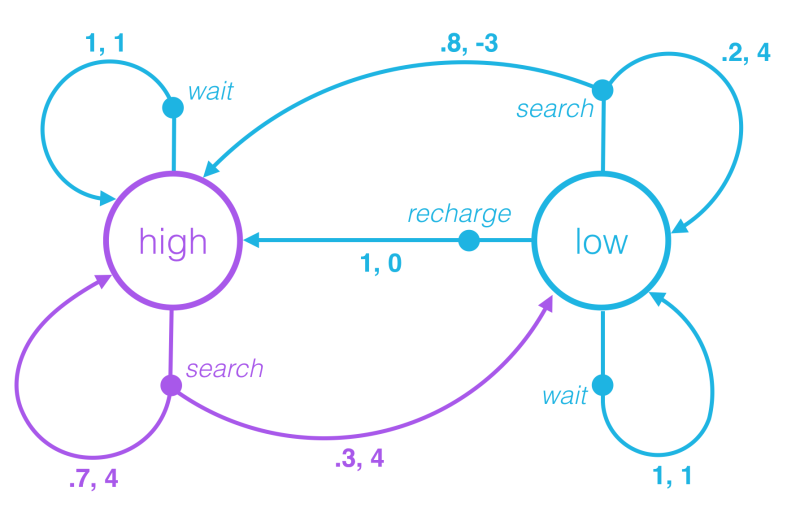
\includegraphics[width=7cm, height=7cm, keepaspectratio]{images/mc_td_1.png}
\end{center}
\end{column}
\end{columns}
\end{frame}

\section{Monte Carlo}

\begin{frame}{Monte Carlo becslés}
\begin{columns}
\begin{column}{.6\textwidth}
\only<1>{A dinamikus programozási algoritmusok futtatásához szükség volt a környezet dinamikájának modelljére. Ez a tulajdonságuk gyakran használhatatlanná teszik őket a gyakorlatban, mert a környezeti dinamika vagy nem ismert vagy nem kiszámítható sok esetben. \par\smallskip
A Monte Carlo (\textbf{MC}) módszerek ezzel szemben nem igényelnek előzetes tudást a feladat elvégzéséhez: csak \textbf{tapasztalat} szükséges ahhoz, hogy megtanuljanak elvégezni egy feladatot. Ezt úgy érik el, hogy mintát vesznek állapotokból, cselekvésekből és jutalmakból, majd az eredményeket átlgolják.}
\only<2>{\begin{center}
\begin{block}{Monte Carlo szimuláció}
Számítási algoritmusok olyan osztálya, ami a véletlen vagy bizonytalan komponens hatását analizálja vagy szimulálja sztochasztikus folyamatokban. 
\end{block}
\end{center}}
\end{column}
\begin{column}{.4\textwidth}
\begin{center}

\includegraphics[width=6cm, keepaspectratio]{images/mc_td_2.png}
\end{center}
\end{column}
\end{columns}
\end{frame}

\begin{frame}{Monte Carlo a megerősítéses tanulásban}
\begin{columns}
\begin{column}{.5\textwidth}
A MC tanítási algoritmus a politika iteráció egy általánosított változata. A megerősítéses tanulásban a MC algoritmusok a mélységi bejárásnak felelnek meg. \par\smallskip
\begin{block}{MC állapot-érték frissítési szabály}
\[
V(s_{t}) \leftarrow V(s_{t}) + \alpha \left[ G_{t} - V(s_{t}) \right]
\]
\vspace{-0.5cm}
\begin{itemize}
	\item $\alpha$: Tanulási sebesség
	\item $G_{t} = \sum_{k=0}^\infty \gamma^k r_{t+k+1}$: Diszkontált kumulált hozam
\end{itemize}
\end{block}
\end{column}
\begin{column}{.5\textwidth}
A központban egy egyszerű ötlet áll: epizódonkénti nyers tapasztalatok alapján tanul anélkül, hogy szüksége lenne a környezet dinamikájának modelljére.
\begin{center}
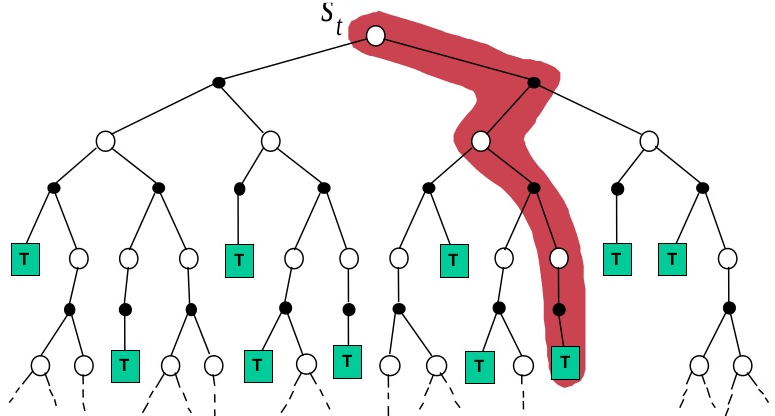
\includegraphics[width=7cm, height=7cm, keepaspectratio]{images/mc_td_3.png}
\end{center}
\end{column}
\end{columns}
\end{frame}

\begin{frame}{Értékfüggvények a Monte Carlo tanításban}
\begin{columns}
\begin{column}{.8\textwidth}
Mivel a MC epizódonként vesz mintát a hozamokból, az értékfüggvények csak sok epizód hozamának átlagolásaként számítódhatnak ki.\par\smallskip
\only<1>{Az \textbf{állapot-érték függvény} megadja, mennyi a várható hozam, ha az ügynök adott $s$ állapotban áll, és onnan $\pi$ politikát követi:
\begin{block}{}
\[
V_{\pi}(s)=Avg\left\{ G_{t:T}|s_{t}=s \right\}
\]
\end{block}}
\only<2>{Az \textbf{állapot-cselekvés minőség függvény} megadja, mennyi a várható hozam, ha az ügynök adott $s$ állapotban áll, $a$ cselekvést végrehajtja, majd onnan $\pi$ politikát követi:
\begin{block}{}
\[
Q_{\pi}(s,a)=Avg \left\{ G_{t:T} | s_{t}=s, a_{t}=a \right\}
\]
\end{block}}
Ahol
\[
G_{t:T}=\sum_{k=0}^{T-t}\gamma^k r_{t+k}
\]
$t$ aktuális időlépéstől a $T$ terminális állapotba vezető időlépésig az ügynök által összegyűjtött diszkontált kumulált hozam.
\end{column}
\begin{column}{.2\textwidth}
\begin{center}
\only<1>{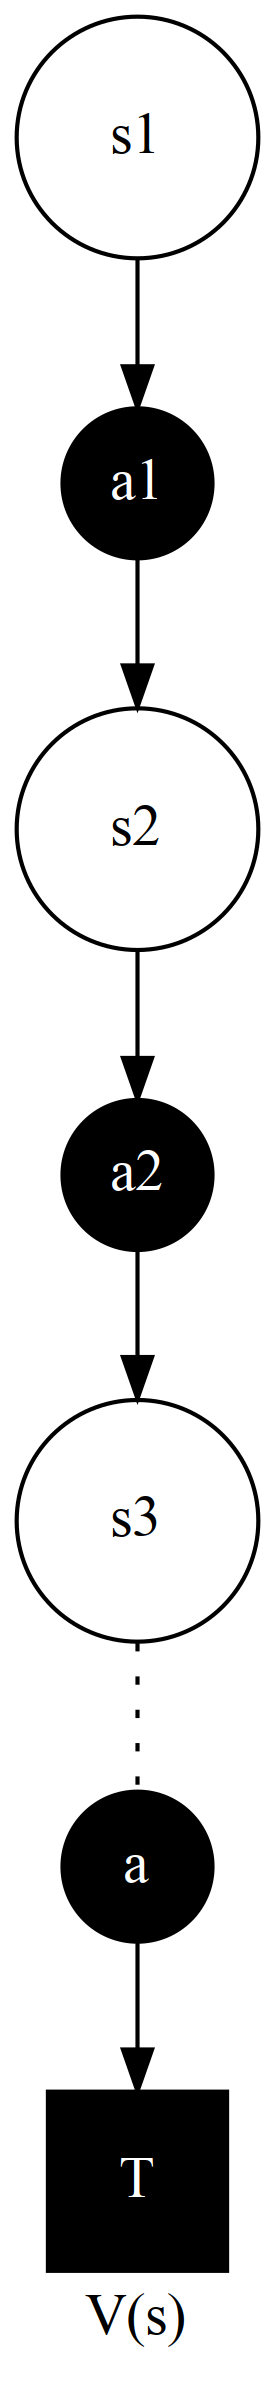
\includegraphics[height=7cm, keepaspectratio]{graphs/mc_td_2.png}}
\only<2>{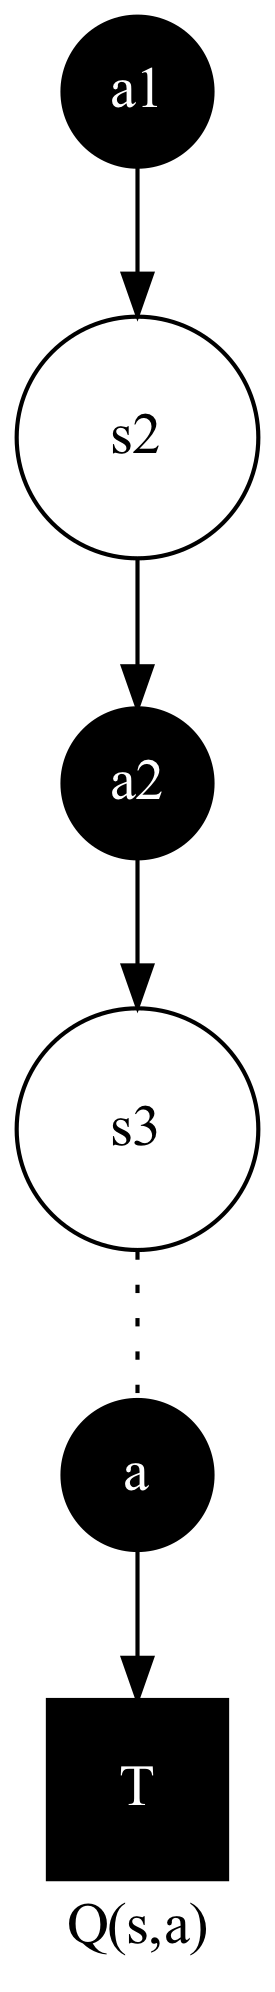
\includegraphics[height=7cm, keepaspectratio]{graphs/mc_td_3.png}}
\end{center}
\end{column}
\end{columns}
\end{frame}

\begin{frame}{MC politika kiértékelés}
\begin{columns}
\begin{column}{.5\textwidth}
\only<1>{A $V_{\pi}(s)$ állapot-érték függvény egy állapotonkénti vektor, amely minden állapot esetén számon tartja az adott $s$ állapotból indulva összegyűjtött jutalmak várható értékét ha az ügynök egy adott $\pi$ politika szerint cselekszik.}
\only<2>{A $Q_{\pi}(s,a)$ állapot-cselekvés minőség függvény egy mátrix, amely az állapot-cselekvés párokhoz tartozóan tárolja el, hogy egy adott $s$ állapotból $a$ cselekvést végrehajtva mennyi a jutalom várható értéke ha az ügynök egy adott $\pi$ politika szerint cselekszik.}
\par\smallskip
Az értékfüggvény \textbf{diszkrét} adatszerkezetben tartja számon a hozamok várható értékét, ezért diszkrét állapotokat és cselekvéseket feltételez.
\end{column}
\begin{column}{.5\textwidth}
\begin{center}
\only<1>{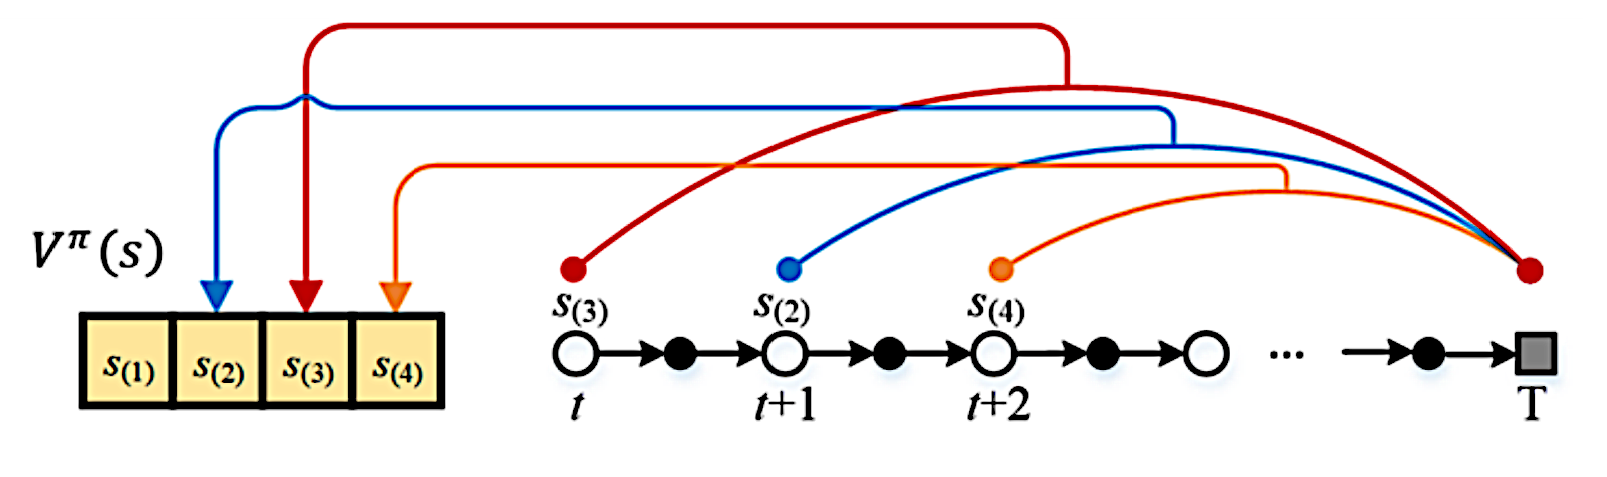
\includegraphics[width=7cm, keepaspectratio]{images/mc_td_4.png}}
\only<2>{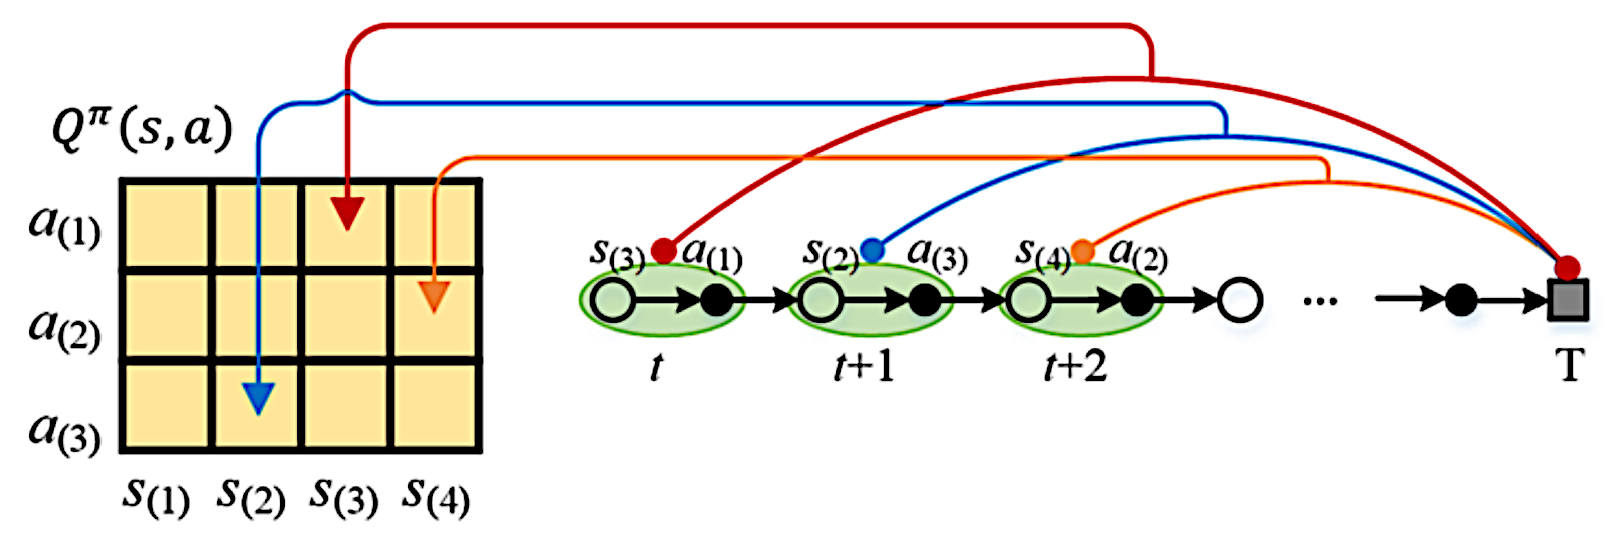
\includegraphics[width=7cm, keepaspectratio]{images/mc_td_5.png}}
\end{center}
\end{column}
\end{columns}
\end{frame}

\begin{frame}{Látogatás alapú Monte Carlo becslés}
\begin{columns}
\begin{column}{.5\textwidth}
Az ügynök-környezet interakció alatt az ügynök egy adott $s$ állapotot többször is meglátogathat egy epizód alatt. Az ábrán ez a $6$-os állapot, amit kétszer látogatott meg az ügynök. \par\smallskip 
Ezt kétféleképpen tudja kezelni az MC algoritmusa: vagy az első látogatást, vagy minden látogatást fog figyelembe venni az értékfüggvények számításakor. Az első látogatás alapú MC esetén csak az első látogatás hozamát fogja figyelembe venni átlagoláskor, míg az összes látogatás alapú esetén mindegyiket.
\end{column}
\begin{column}{.5\textwidth}
Mindkét esetben a valós értékhez való konvergencia garantált, ahogy a látogatások száma közelít a $\infty$-hez. 
\begin{center}
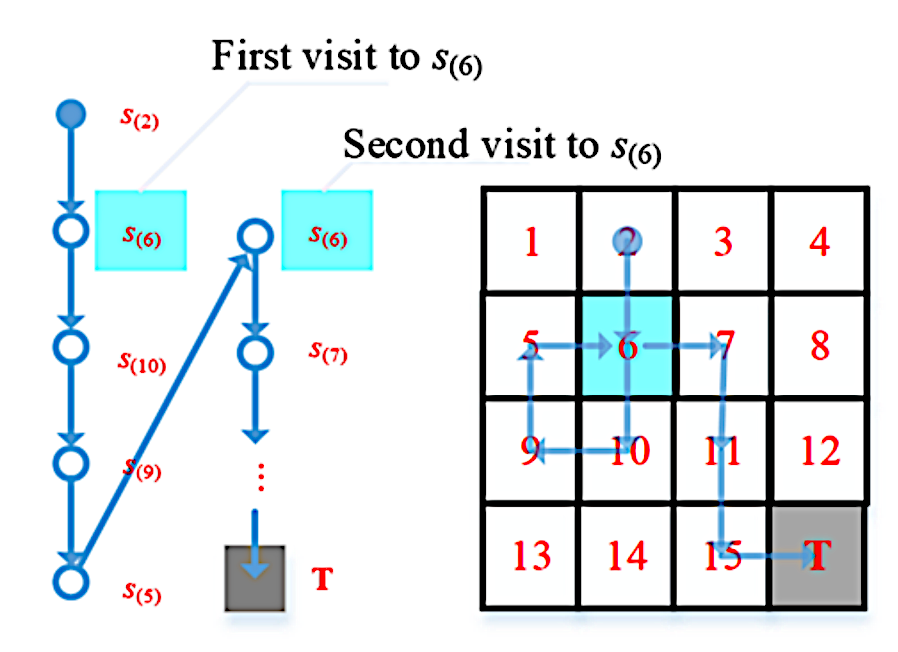
\includegraphics[width=7cm, keepaspectratio]{images/mc_td_6.png}
\end{center}
\end{column}
\end{columns}
\end{frame}

\begin{frame}{}
\begin{algorithm}[H]
\caption{Első látogatás alapú Monte Carlo algoritmus $v_{\pi}$ becslésére}
\SetAlgoLined
\textbf{Input:} A kiértékelendő $\pi$ politika\par\smallskip
$V(s) \leftarrow random()$, minden $s \in S$-re\;
$Hozam(s) \leftarrow $ \textbf{üres lista}, minden $s \in S$-re\; 
\For{$i=0 \rightarrow max_i$}{
	Epizód lejátszása $\pi$ politikával: $s_0, a_0, r_1, s_1, a_1, r_2, ..., s_{T-1}, a_{T-1}, r_T$\;
	$G \leftarrow 0$\tcc*[t]{Hozam inícializálása $0$ értékkel}
	\For{$t=T-1 \rightarrow 0$}{
		$G \leftarrow \gamma G+R_{t+1}$\tcc*[t]{Hozam diszkontálása és kumulálása}
		\If{$s_t$ \textbf{not in} $s_0, s_1, ..., s_{t-1}$}{
			$G$ hozzáfűzése $Hozam(s_t)$-hez\tcc*[t]{Állapothoz tartozó hozam}
			$V(s_t) \leftarrow Avg \left\{ Hozam(s_t) \right\}$\tcc*[t]{Hozam várható értéke}
		}
	}
}
\end{algorithm}
\end{frame}

\begin{frame}{}
\begin{algorithm}[H]
\caption{Monte Carlo becslés $\pi_{*}$ keresésére}
\SetAlgoLined
\begin{small}
$\pi(s) \in A(s)$ véletlenszerűen, minden $s \in S$-re\;
$Q(s,a) \in \mathbb{R}$ véletlenszerűen, minden $s \in S$-re és $a \in A$-ra\;
$Hozam(s,a) \leftarrow$ üres lista minden $s \in S$-re és $a \in A$-ra\;
\For{$i=0 \rightarrow max_i$}{
	$s_0 \in S$ és $a_0 \in A$ véletlenszerű kiválasztása\;
	Epizód lejátszása $s_0, a_0$-ból $\pi$ politikával: $s_0, a_0, r_1, s_1, a_1, r_2, ..., s_{T-1}, a_{T-1}, r_T$\;
	$G \leftarrow 0$\tcc*[t]{Hozam inícializálása $0$ értékkel}
	\For{$t=T-1 \rightarrow 0$}{
		$G \leftarrow \gamma G+R_{t+1}$\tcc*[t]{Hozam diszkontálása és kumulálása}
		\If{$\left(s_t, a_t \right)$ \textbf{not in} $s_0, s_1, ...s_{t-1}$}{
			$G$ hozzáfűzése $Hozam(s_t,a_t)$-hez\tcc*[t]{Állapot-cselekvés pár hozama}
			$Q(s_t, a_t) \leftarrow Avg \left\{ Hozam(s_t, a_t) \right\}$\tcc*[t]{Hozam várható értéke}
			$\pi(s_t) \leftarrow \underset{a}{argmax}Q(s_t, a)$\tcc*[t]{Politika frissítése}
		}
	}
}
\end{small}
\end{algorithm}
\end{frame}

\begin{frame}{Példa: Monte Carlo értékbecslés egy látogatás esetén}
\begin{columns} % https://towardsdatascience.com/monte-carlo-learning-b83f75233f92
\begin{column}{.5\textwidth}
Az ügynök 3 tanítási iteráción keresztül játszott. Minden esetben a a végállapot $s_T=s_{13}$. Ez 3 tanítási mintának felel meg:
\begin{scriptsize}
\[
Hozam(01) = \underset{s_{05}}{2}+\underset{s_{04}}{1}+\underset{s_{07}}{2}+\underset{s_{10}}{2}+\underset{s_{11}}{1}+\underset{s_{13}}{5}=13
\]
\[
Hozam(02) = \underset{s_{05}}{2}+\underset{s_{06}}{3}+\underset{s_{08}}{1}+\underset{s_{12}}{3}+\underset{s{11}}{1}+\underset{s_{13}}{5}=15
\]
\[
Hozam(03) = \underset{s_{05}}{2}+\underset{s_{06}}{3}+\underset{s_{08}}{1}+\underset{s_{12}}{3}+\underset{s_{11}}{1}+\underset{s_{13}}{5}=15
\]
\end{scriptsize}
Tehát a megfigyelt átlagos hozam $s_{05}$ állapotból indulva: 
\[
V_\pi(s_{05})=\frac{13+15+15}{3}=14.33
\]
Megjegyzés: $\gamma=1$
\end{column}
\begin{column}{.5\textwidth}
\begin{center}
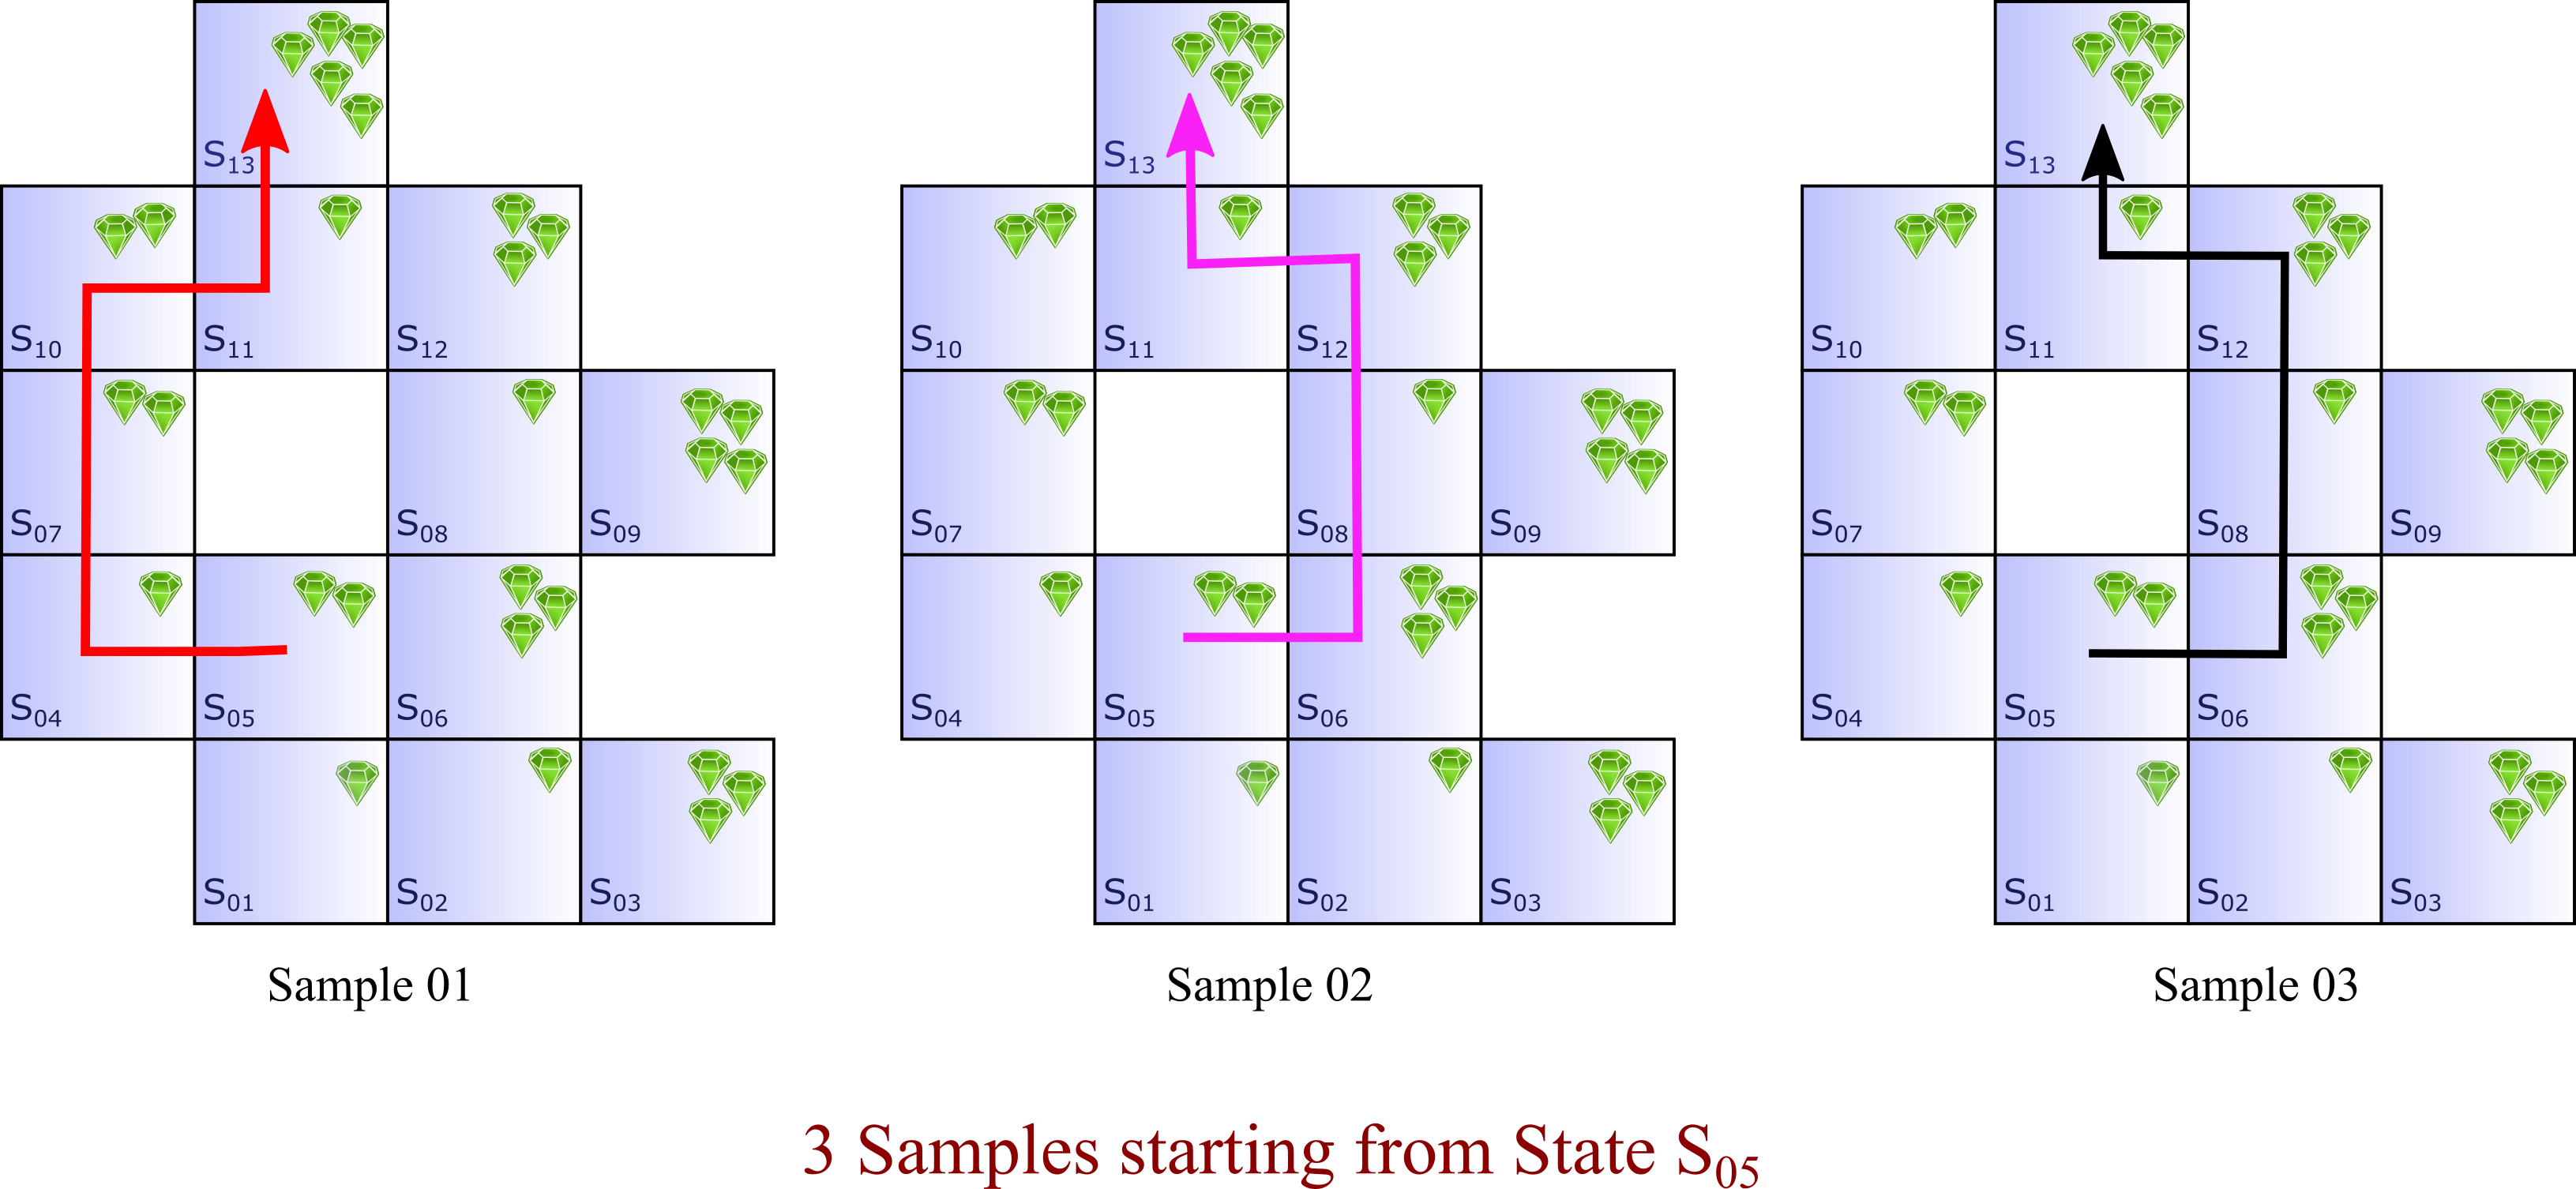
\includegraphics[width=7cm, keepaspectratio]{images/mc_td_12.png}
\end{center}
\end{column}
\end{columns}
\end{frame}

\begin{frame}{Példa: Monte Carlo értékbecslés több látogatás esetén}
\begin{columns}
\begin{column}{.5\textwidth}
Ha az ügynök többször látogatta meg ugyanazt az állapotot a tanítási iterációk során, a tanítási iteráció során kezelni kell a több látogatásból adódó jutalom többletet. Az első látogatás alapú MC tanulás során az ügynök első látogatásától a jutalom kumulálodva számítódik.\par\smallskip
Ebben az esetben $s_{05}$ állapot értéke:
\[
V_\pi(s_{05})=\frac{33+15+15}{3}=21
\]
Megjegyzés: $\gamma=1$ 
\end{column}
\begin{column}{.5\textwidth}
\begin{center}
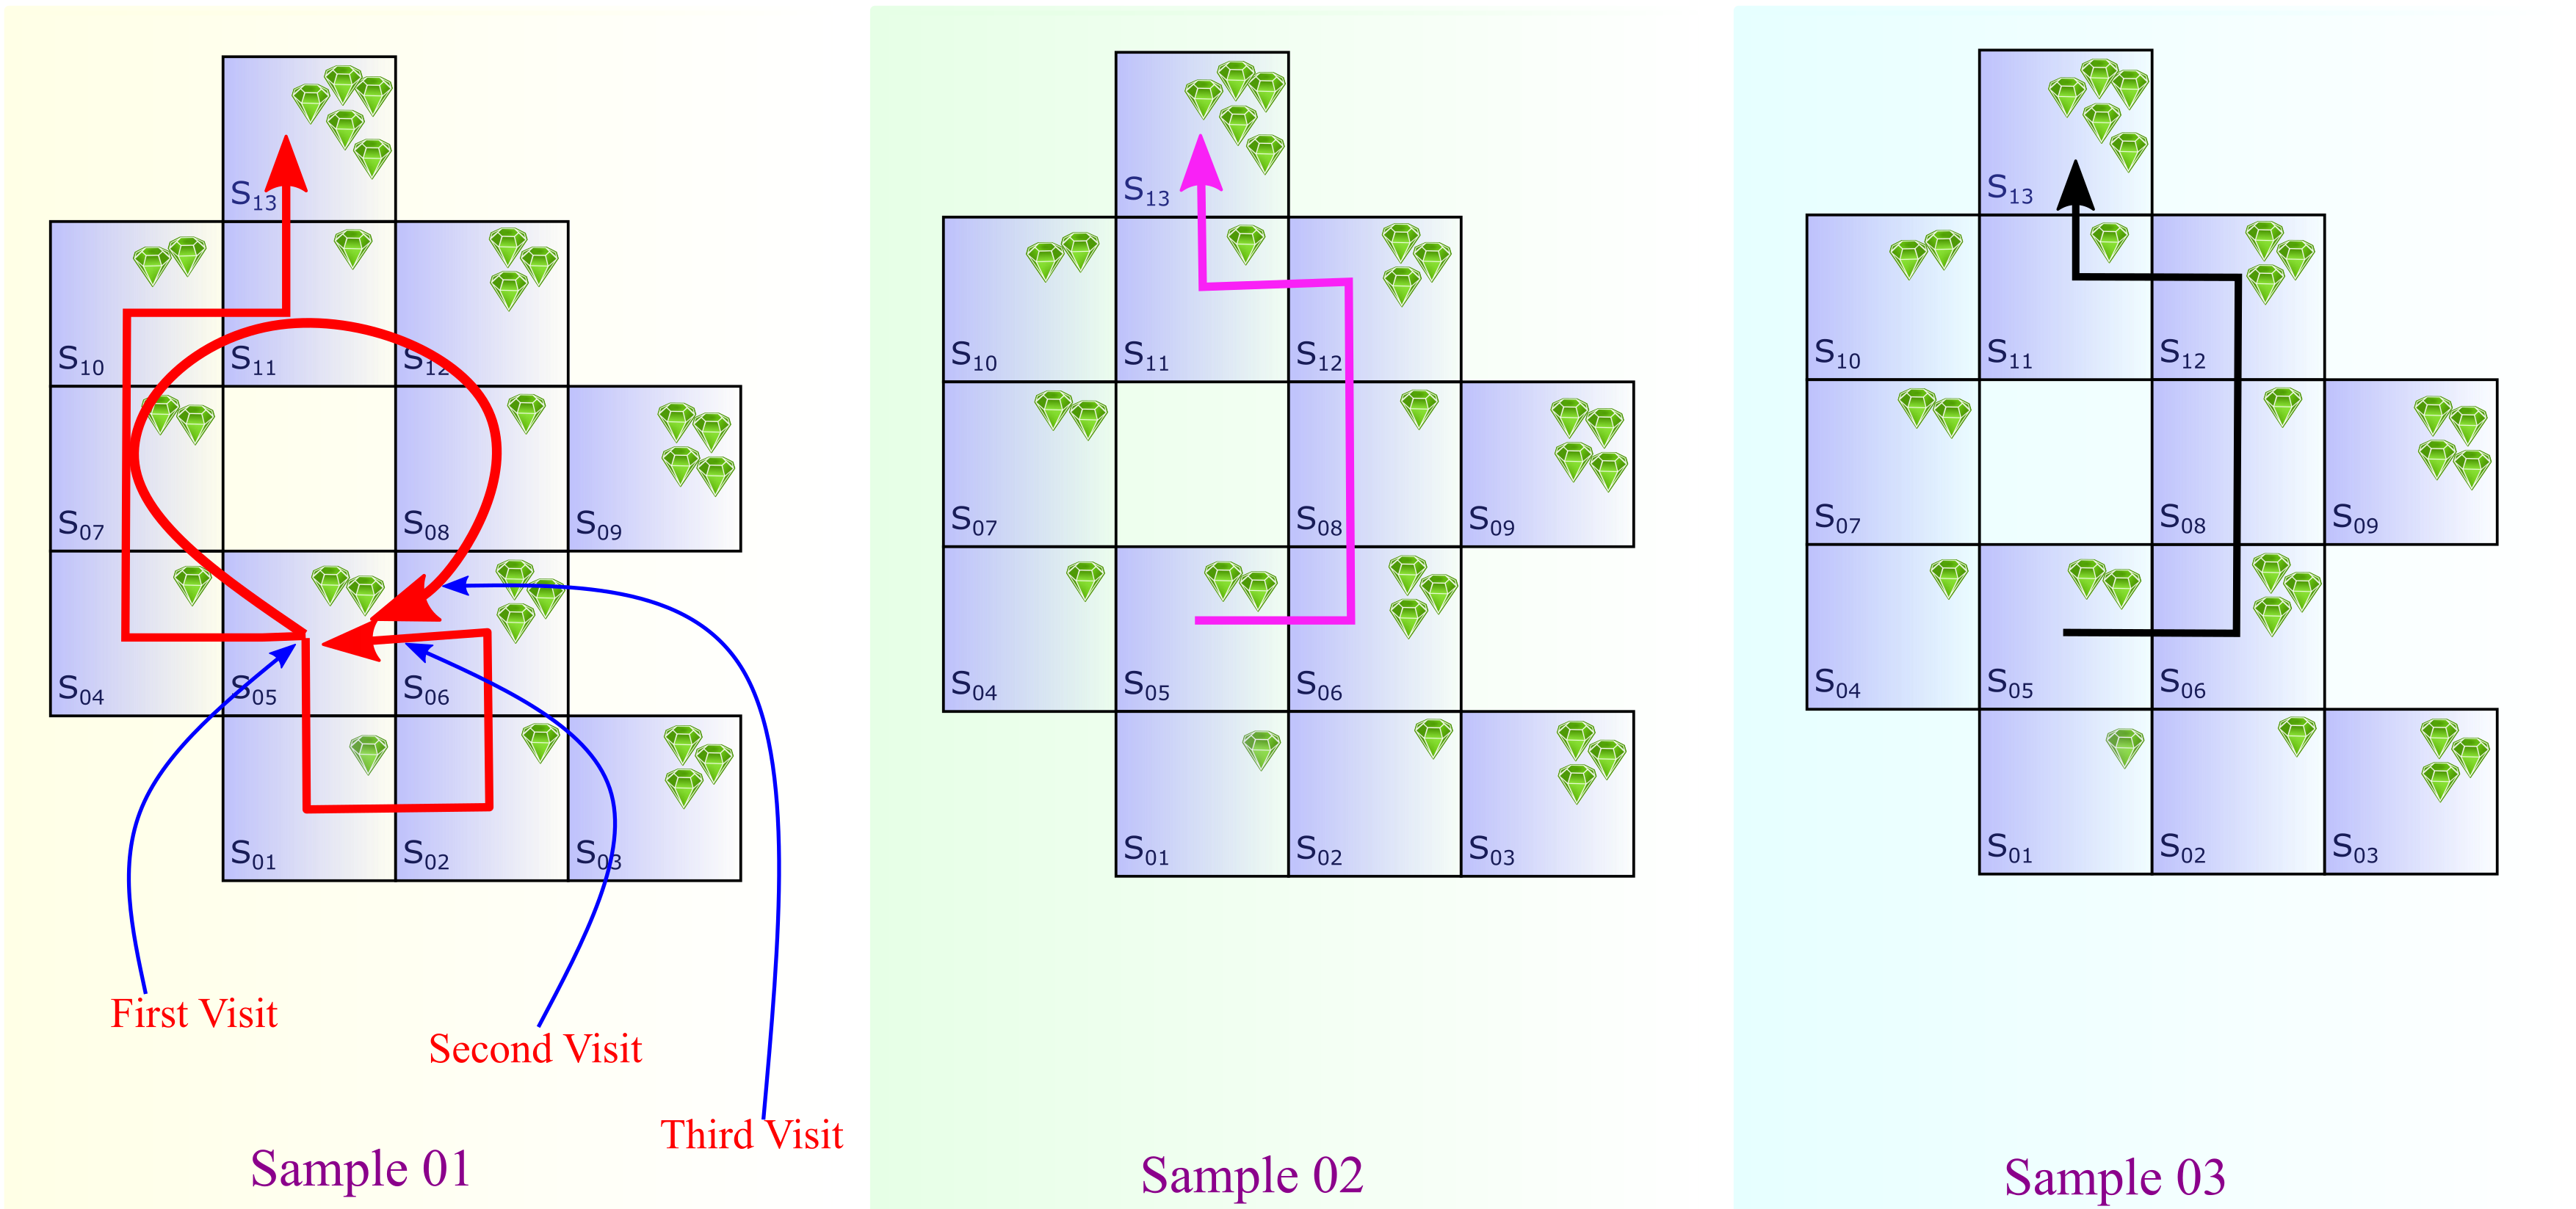
\includegraphics[width=7cm, keepaspectratio]{images/mc_td_13.png}
\end{center}
\end{column}
\end{columns}
\end{frame}

\section{Időbeli különbségek}

\begin{frame}
\tableofcontents[currentsection]
\end{frame}

\begin{frame}{Időbeli különbségek}
\begin{columns}
\begin{column}{.5\textwidth}
Az egyik központi ötlete a megerősítéses tanulásnak az időbeli különbségek (\textbf{TD}) tanító algoritmusa. A TD kombinálja a MC és DP algoritmusok ötleteit. \par\smallskip
Csakúgy mint a MC, nyers tapasztalatokból tud tanulni, ezért \textbf{nincs szüksége a környezet dinamikájának modelljére}. És hasonlóan a DP algoritmusokhoz, az ügynöknek \textbf{nem szükséges teljes epizódokat lejátszania}.
\end{column}
\begin{column}{.5\textwidth}
\begin{center}
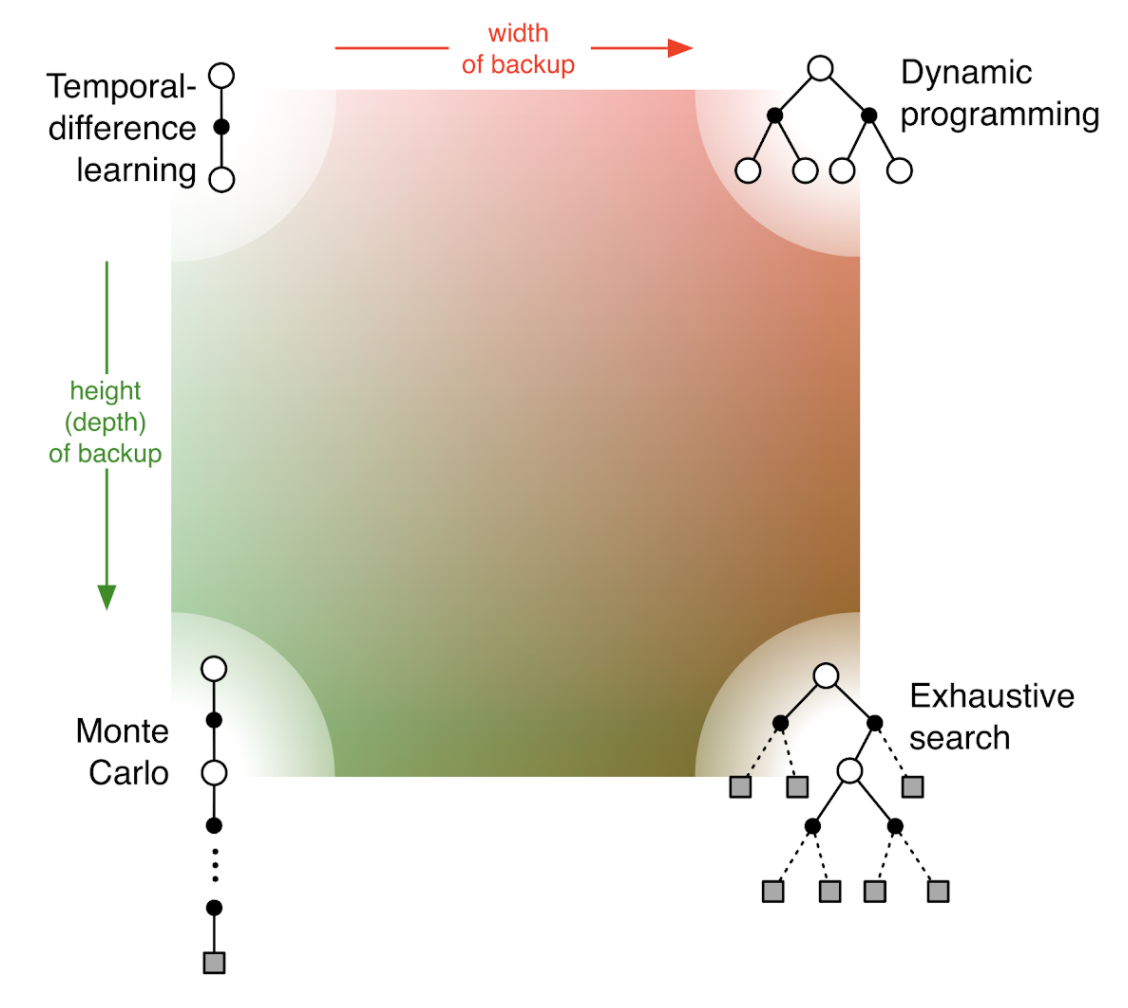
\includegraphics[width=7cm, keepaspectratio]{images/mc_td_7.png}
\end{center}
\end{column}
\end{columns}
\end{frame}

\begin{frame}{TD becslés}
\begin{columns}
\begin{column}{.7\textwidth}
Az ábrán az időbeli különbségek frissítési diagramja látható. Az $s_1$ állapothoz tartozó állapot-érték csak a következő állapot és a következő állapothoz tartozó jutalom alapján frissül. \par\smallskip
A TD tanítás csak az egyes lépések által kapott jutalomból vesz mintát, és ez alapján számítja ki adott állapotonként a hozamok várható értékét. Az MC és TD becslés a \textbf{mintavevő frissítések} algoritmusainak körébe tartoznak, mert ahhoz, hogy ki lehessen számolni, előre meg kell ismerni a következő állapothoz (vagy állapotokhoz) tartozó jutalmakat.\par\smallskip
A DP algoritmusok esetén nem mintavétel történik, hanem egy teljes sokaság alapján egy várható érték számolódik ki.
\end{column}
\begin{column}{.3\textwidth}
\begin{center}
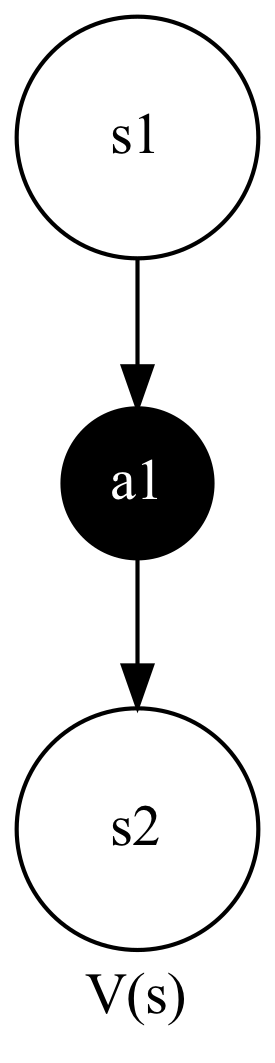
\includegraphics[height=7cm, keepaspectratio]{graphs/mc_td_4.png}
\end{center}
\end{column}
\end{columns}
\end{frame}

\begin{frame}{TD a megerősítéses tanulásban}
\begin{columns}
\begin{column}{.55\textwidth}
\begin{block}{TD állapot-érték frissítési szabály}
\[
V(s) \leftarrow V(s) + \alpha \left[ r + \gamma V(s') - V(s) \right]
\]
\vspace{-0.5cm}
\begin{itemize}
	\item $\alpha$: Tanulási sebesség
	\item $r$: Jutalom
\end{itemize}
\end{block}
A zárójelben lévő kifejezés a \textbf{TD hiba}, ami a $s_t$ jelen állapot értéke és a jobb becslés, $r + \gamma V(s')$ közötti távolságot adja meg. A megerősítéses tanulásban számos helyen jelen van: 
\[
\delta_t=r + \gamma V(s') - V(s)
\]
\end{column}
\begin{column}{.5\textwidth}
\begin{center}
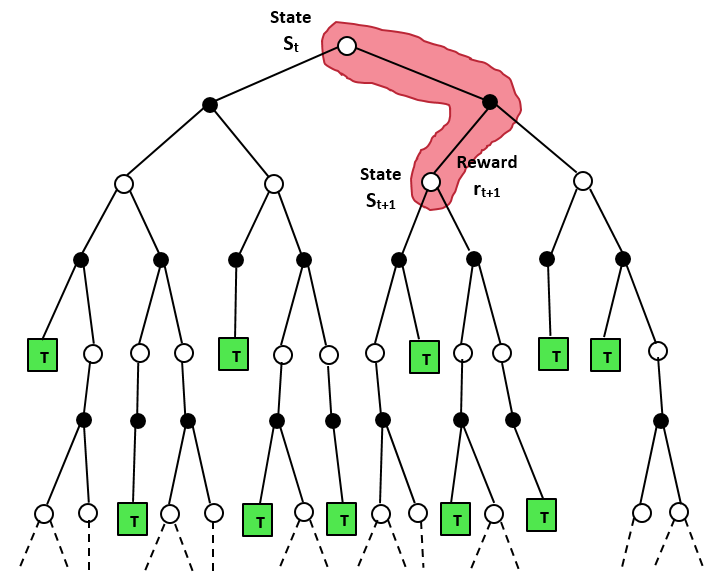
\includegraphics[width=7cm, keepaspectratio]{images/mc_td_8.png}
\end{center}
\end{column}
\end{columns}
\end{frame}

\begin{frame}{}
\begin{algorithm}[H]
\caption{TD algoritmus $v_\pi$ megbecslésére}
\SetAlgoLined
\textbf{Input}: $\pi$ politika ami kiértékelésre kerül; $\alpha \in [0,1]$ tanulási sebesség\par\smallskip
$V(s) \leftarrow random()$, minden $s \in S$-re\tcc*[t]{Állapot-értékek inícializálása}
$V(s_T) \leftarrow 0$\tcc*[t]{Terminális állapot értékének 0-ra állítása}
\For{$i=0 \rightarrow max_i$}{
	$s \leftarrow s_0$\tcc*[t]{Kezdőállapot felvétele}
	\While{$s \neq s_T$}{
		$a \leftarrow \pi(s)$\tcc*[t]{Cselekvés választás $s$ állapotból $\pi$ szerint}
		$a$ végrehajtása, $r, s'$ megfigyelése\;
		$V(s) \leftarrow V(s) + \alpha \left[ r + \gamma V(s') - V(s) \right]$\;
		$s \leftarrow s'$\tcc*[t]{Aktuális állapot frissítése}
	}
}
\end{algorithm}
\end{frame}

\begin{frame}{Példa TD becslésre}
A robot célja eljutni a bal alsó kockáról a zöld kockára jutalomért. Ha a piros kockára lép negatív jutalmat kap. Az ábrán egy epizód eredménye látható.
\begin{columns}
\begin{column}{.5\textwidth}
\begin{center}
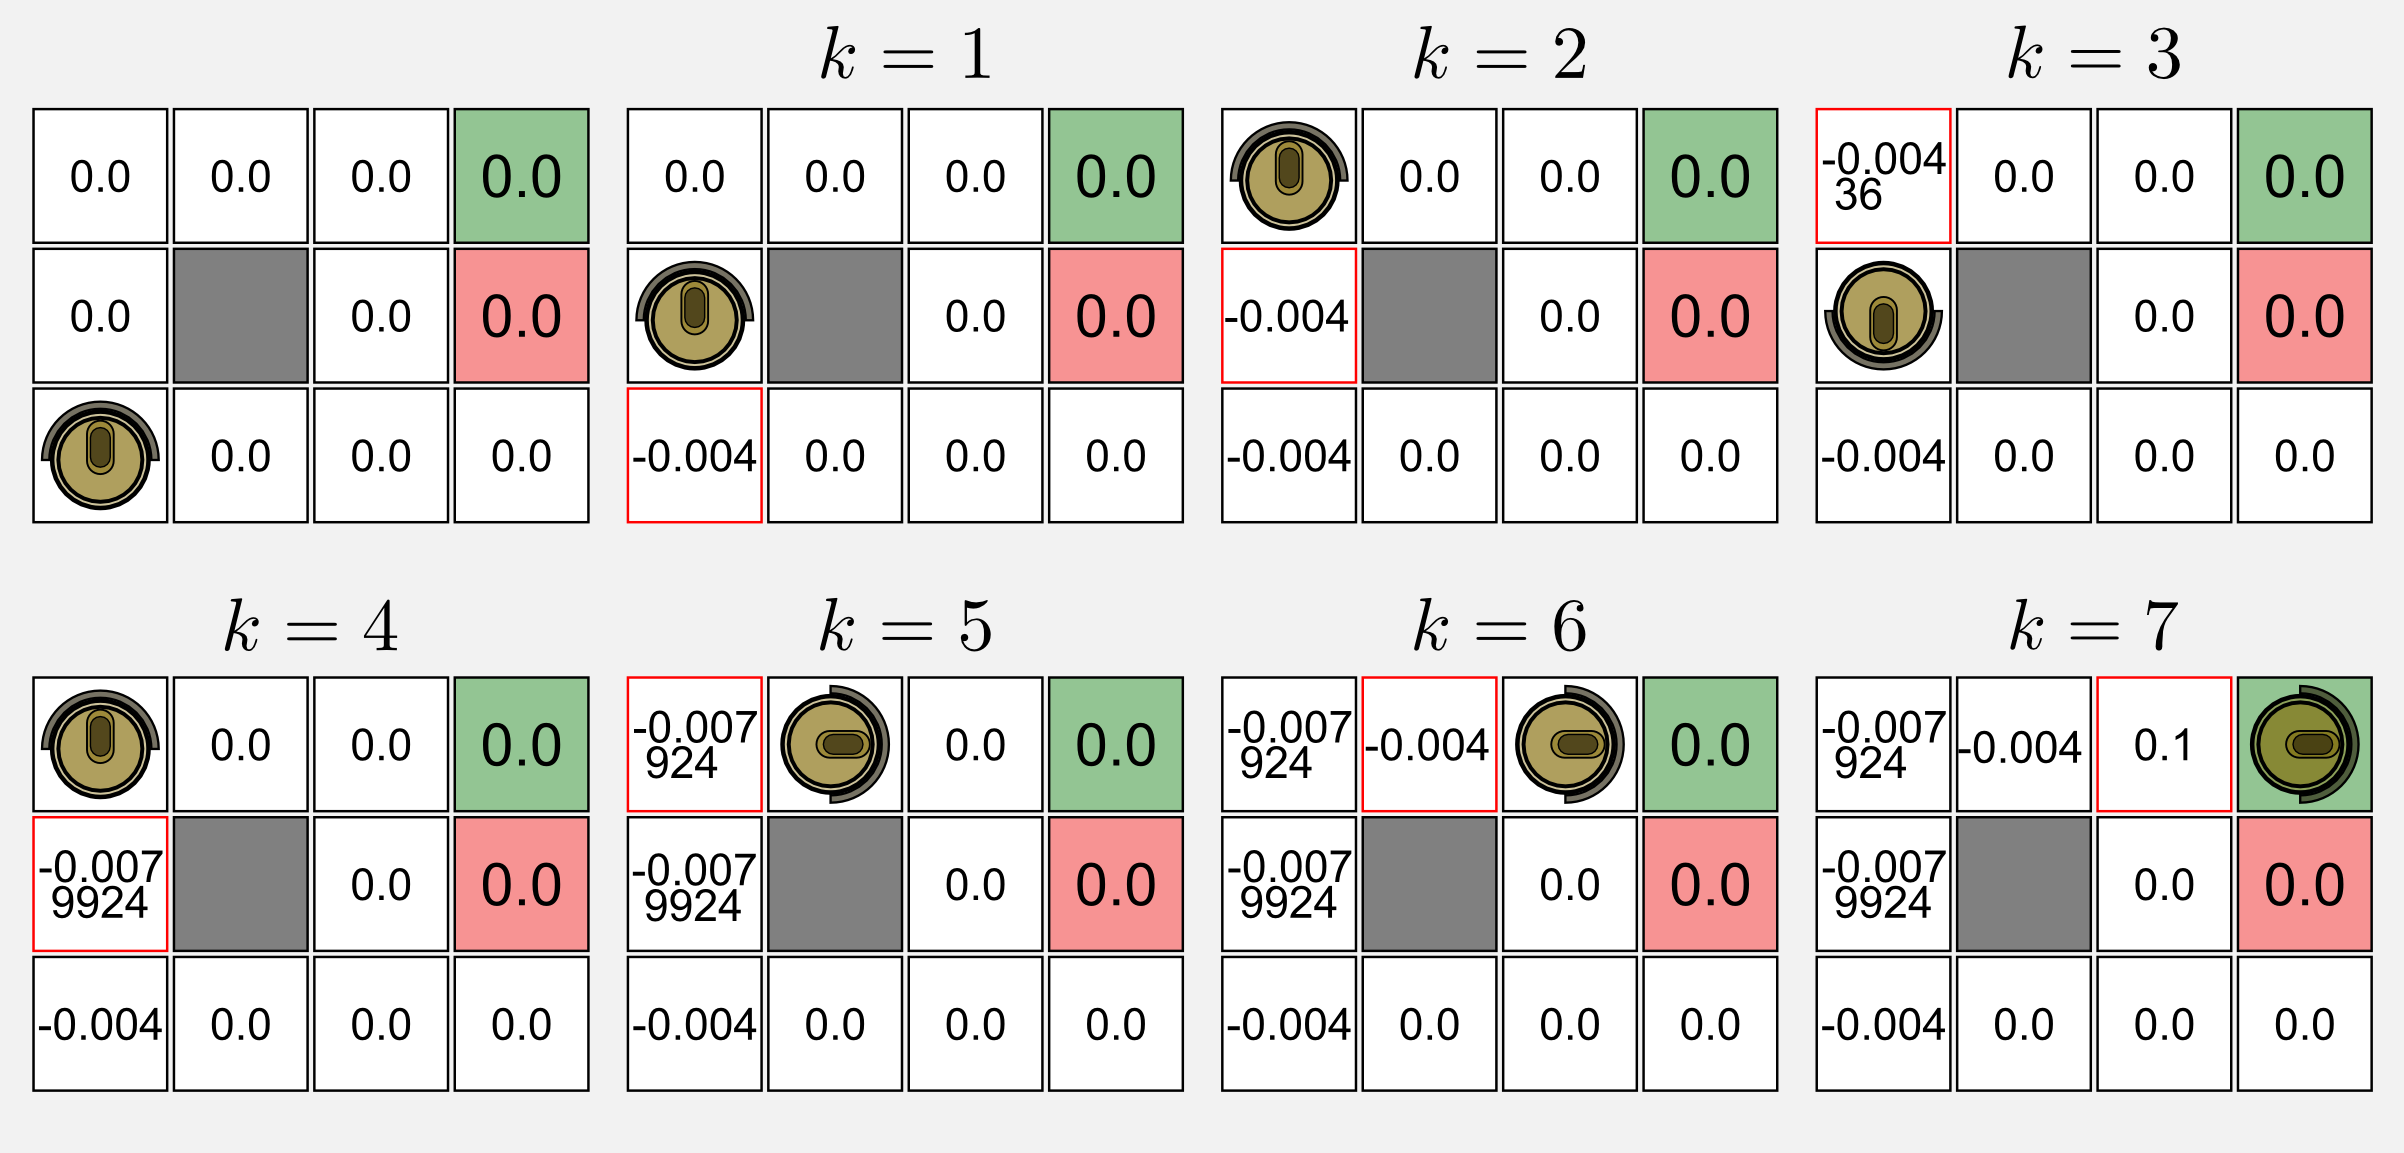
\includegraphics[width=7cm, keepaspectratio]{images/mc_td_17.png}
\end{center}
\end{column}
\begin{column}{.5\textwidth}
\begin{center}
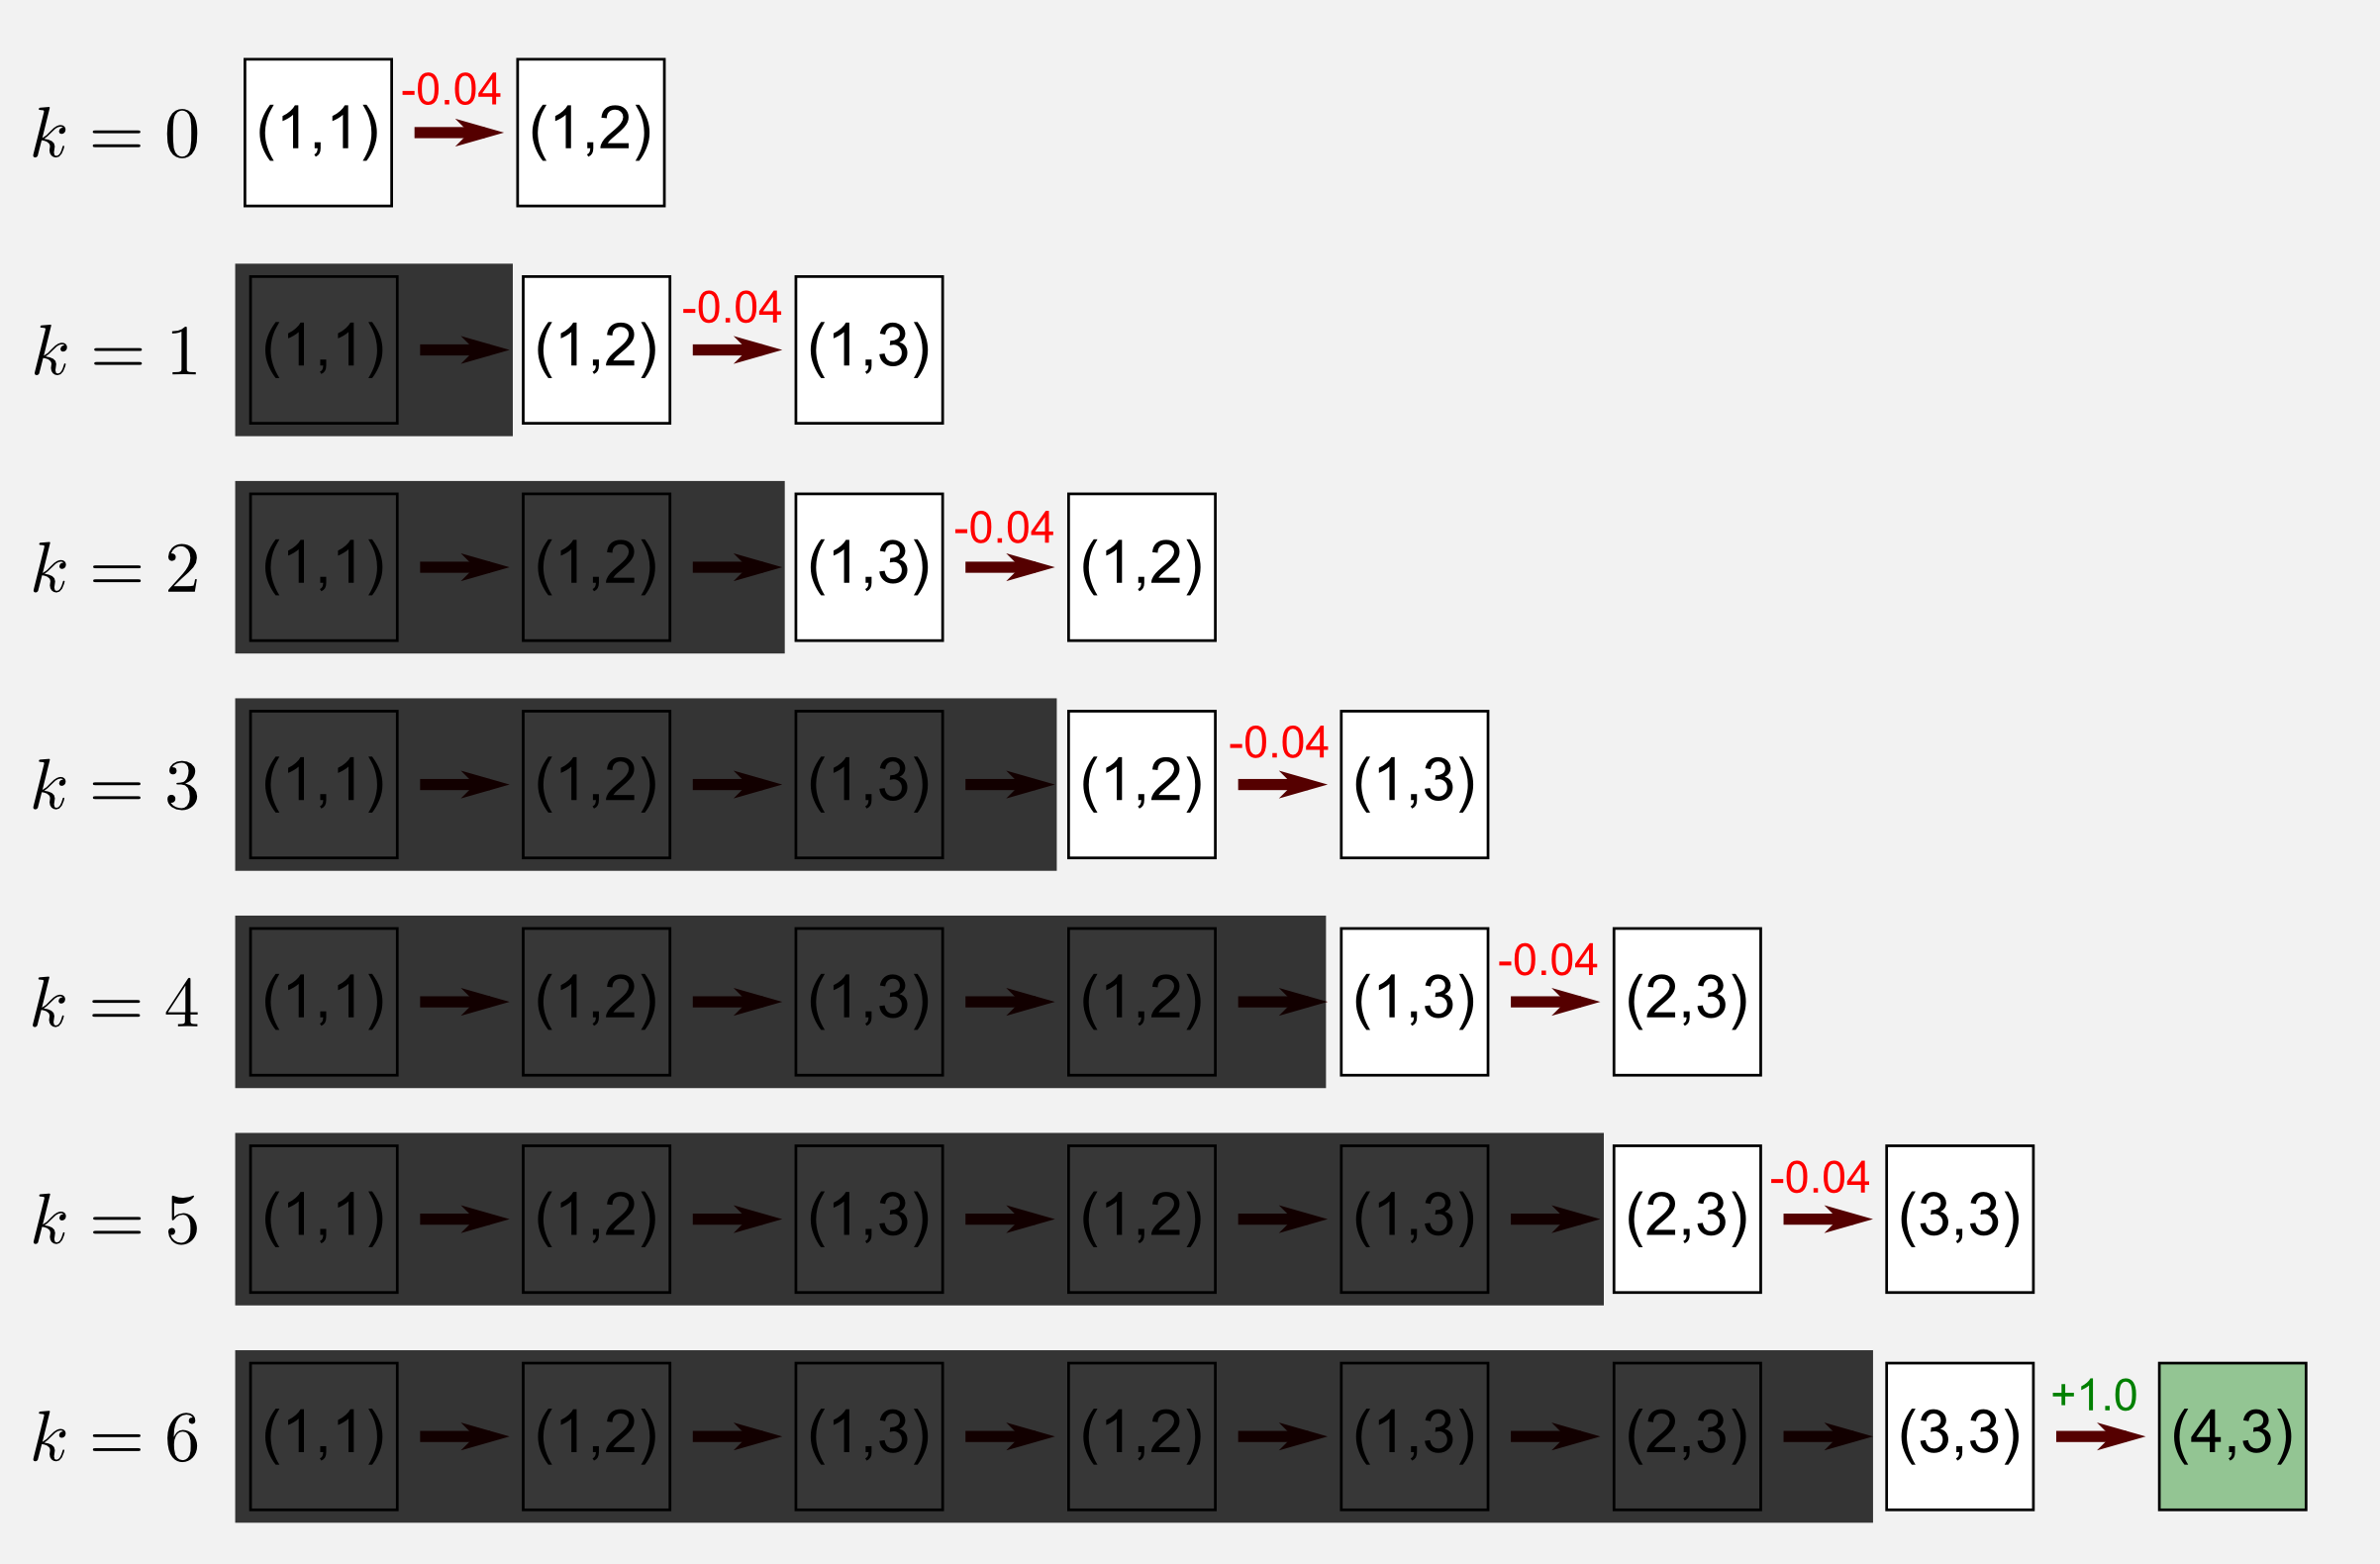
\includegraphics[width=7cm, keepaspectratio]{images/mc_td_18.png}
\end{center}
\end{column}
\end{columns}
\end{frame}

\section{SARSA}

\begin{frame}
\tableofcontents[currentsection]
\end{frame}

\begin{frame}{Politikaalapú TD irányítás: SARSA}
\begin{columns}
\begin{column}{.8\textwidth}
TD becsléssel lehetséges a $v_\pi$ mellett a $q_\pi$ értékfüggvény is. Ebben az esetben nem állapot-állapot átmeneteket hanem állapot-cselekvés állapot-cselekvés átmeneteket tanul az algoritmus. \textbf{Formálisan mindkettő Markov folyamat} jutalmazási rendszerrel. \par\smallskip
\begin{center}
\begin{block}{SARSA frissítési szabálya}
\[
Q(s,a) \leftarrow Q(s,a) + \alpha \left[ r + \gamma Q(s',a') - Q(s,a) \right]
\]
\vspace{-0.5cm}
\begin{itemize}
	\item $Q(s,a)$: $s$ állapot és $a$ cselekvés minőség függvénye $t$ időlépésben
	\item $Q(s',a')$: a következő állapot és cselekvés minőség függvénye $t+1$ időlépésben
\end{itemize}
\end{block}
\end{center}
\end{column}
\begin{column}{.2\textwidth}
\begin{center}
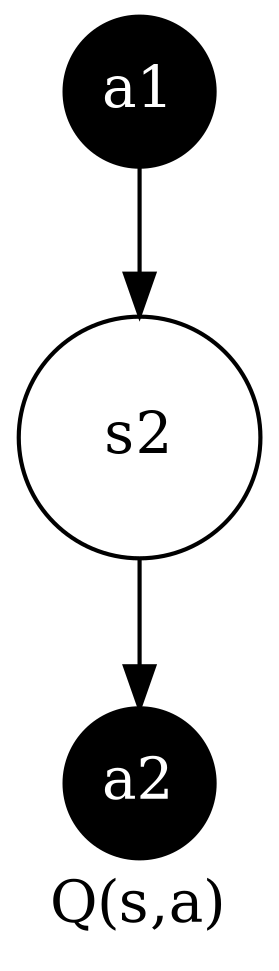
\includegraphics[height=7cm, keepaspectratio]{graphs/mc_td_5.png}
\end{center}
\end{column}
\end{columns}
\end{frame}

\begin{frame}{A SARSA folyamat modellje}
\begin{columns}
\begin{column}{.5\textwidth}
A SARSA frissítési szabálya szerint a tanítási epizód minden lépése alkalmával \textbf{politika kiértékelés} fog végrehajtódni, amikor egy $(s,a,r,s',a')$ sorozattal találkozik a modell. Ha gyakoribb a mintavétel nagyobb a számításigény, viszont pontosabb is a becslés.\par\smallskip
A \textbf{politika javítás} lépésében amikor az ügynök cselekvést választ gyakori az $\varepsilon$-mohó stratégia alkalmazása, ezzel is ösztönözve a felfedezést és nem vélt magas jutalmak megszerzését.
\end{column}
\begin{column}{.5\textwidth}
\begin{center}
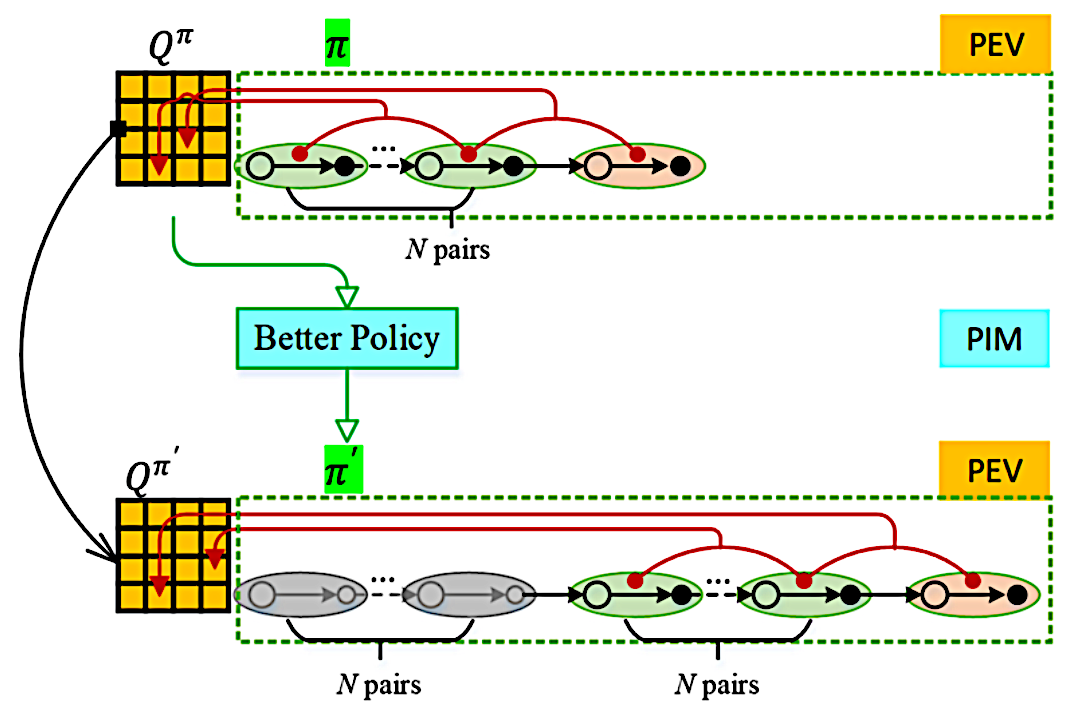
\includegraphics[width=7cm, keepaspectratio]{images/mc_td_10.png}
\end{center}
\end{column}
\end{columns}
\end{frame}

\begin{frame}{SARSA algoritmusa}
\begin{algorithm}[H]
\caption{SARSA algoritmus $Q \approx q_*$ megbecslésére}
\SetAlgoLined
\textbf{Input}: $\alpha$: tanulási sebesség; $\varepsilon > 0$: algoritmus hibahatára\par\smallskip
$Q(s,a) \leftarrow random()$, minden $s \in S$-re és $a \in A$-ra\;
$Q(s_t,\cdot) \leftarrow 0$\tcc*[t]{Terminális állapot értéke $0$}
\For{$i=0 \rightarrow max_i$}{
	$s \leftarrow s_0$\tcc*[t]{Kezdőállapot felvétele}
	$a \leftarrow \pi(s)$\tcc*[t]{Cselekvés választása $s$ állapotból $\pi$ szerint}
	\While{$s \neq s_T$}{
		$a$ végrehajtása, $r, s'$ megfigyelése\;
		$a' \leftarrow \pi(s')$\tcc*[t]{Cselekvés választása $s'$ állapotból $\pi$ szerint}
		$Q(s,a) \leftarrow Q(s,a) + \alpha \left[ r + \gamma Q(s',a') - Q(s,a) \right]$\;
		$s \leftarrow s'$, $a \leftarrow a'$\tcc*[t]{Jelenlegi állapot és cselekvés frissítése}
	}	
}
\end{algorithm}
\end{frame}

\section{$n$-lépéses különbségek}

\begin{frame}
\tableofcontents[currentsection]
\end{frame}

\begin{frame}{MC és TD egyesítése}
\begin{columns}
\begin{column}{.5\textwidth}
A MC eljárások az aktuális állapottól egészen \textbf{az epizód végéig} megfigyelt állapotok alapján számolják ki az új $v_\pi(s)$ értéket.\par\smallskip
A TD módszer pedig \textbf{csak a következő állapotig} kapott jutalom alapján frissíti az értékfüggvényt.\par\smallskip
A köztes módszer, hogy az algoritmus $n$ \textbf{köztes állapotból} származó jutalmat vegye figyelembe. Például ha $n=2$ akkor következő $2$ állapot és a hozzájuk tartozó jutalom ami számít.
\end{column}
\begin{column}{.5\textwidth}
\begin{center}
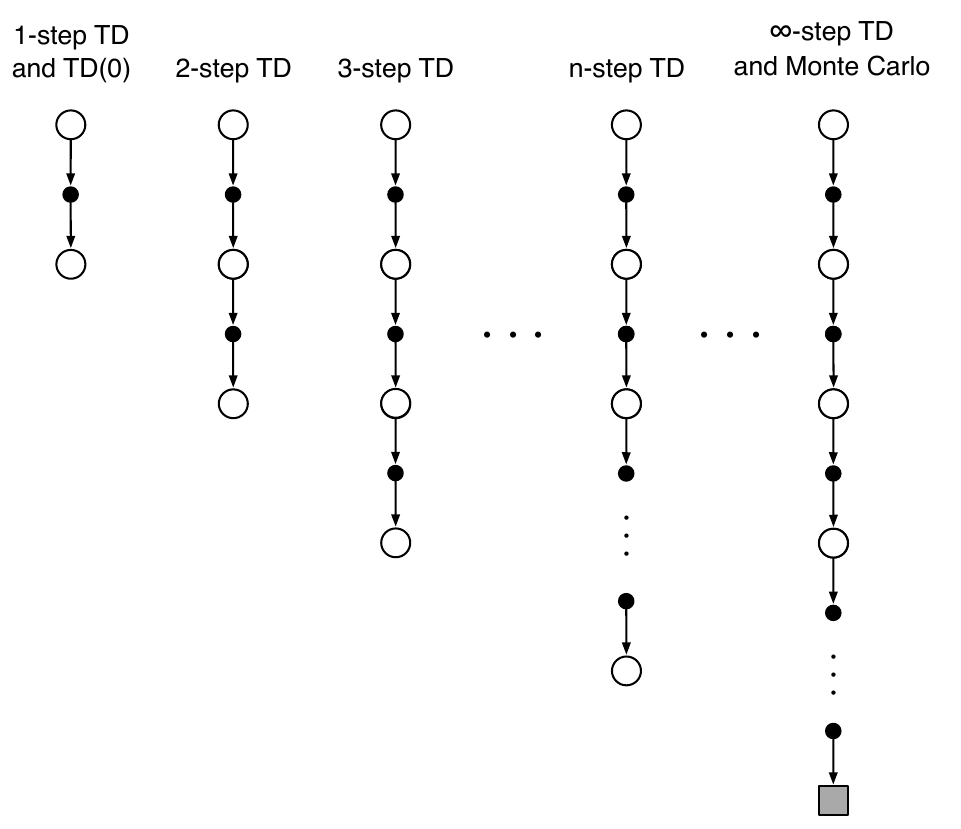
\includegraphics[width=7cm, keepaspectratio]{images/mc_td_14.png}
\end{center}
\end{column}
\end{columns}
\end{frame}

\begin{frame}{TD($n$) értékfüggvényei}
\only<1>{\begin{block}{$n$ lépéses diszkontált hozam}
\begin{center}
$G_{t:t+n}=r_{t+1}+ \gamma r_{t+2}+ ... + \gamma^{n-1}r_{t+n} + \gamma^n V_{t+n-1}(s_{t+n})$
\end{center}
A hozam végén az utolsó, $t+n-1$-edik állapot állapot-értéke szerepel, ezzel kompenzálva az összes, $n$-edik állapot után szereplő állapot várható hozamáért.
\end{block}}
\only<2>{\begin{block}{$n$ lépéses állapot-érték frissítési szabály}
\begin{center}
$V_{t:t+n}=V_{t+n-1}(s_{t}) + \alpha \left[ G_{t:t+n}-V_{t+n-1}(s_{t}) \right]$
\end{center}
Megegyezik az eddig vizsgált állapot-érték függvénnyel kivéve, hogy az $n$ lépéses diszkontált hozamot használja a teljes hozam helyett.
\end{block}}
\only<3>{\begin{block}{$n$ lépéses SARSA}
\begin{center}
$Q_{t+n}(s_t,a_t)=Q_{t+n-1}(s_t,a_t) + \alpha \left[ G_{t:t+n} - Q_{t+n-1}(s_t, a_t) \right]$
\end{center}
Megegyezik az eddig vizsgált állapot-cselekvés minőség függvénnyel kivéve, hogy az $n$ lépéses hozamot használja a teljes hozam helyett.
\end{block}}
\begin{center}
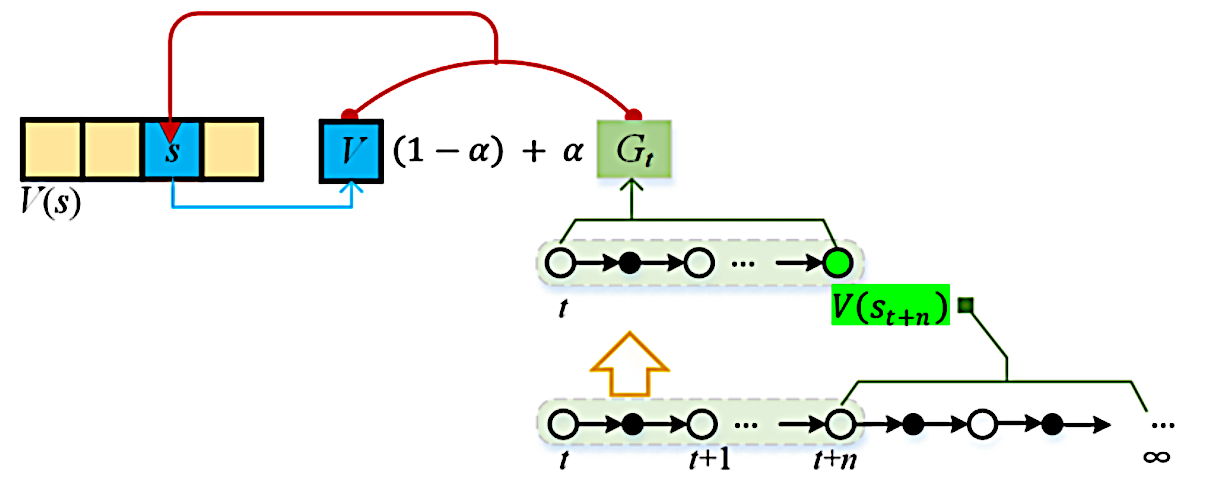
\includegraphics[width=8cm, keepaspectratio]{images/mc_td_15.png}
\end{center}
\end{frame}

\section{Összefoglalás}

\begin{frame}
\tableofcontents[currentsection]
\end{frame}

\begin{frame}{Keresés mélysége}
\begin{center}
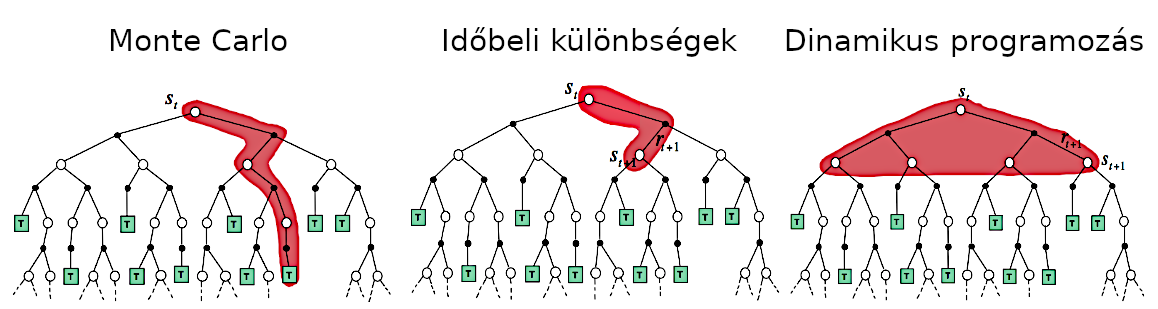
\includegraphics[width=14cm, keepaspectratio]{images/mc_td_11.png}
\end{center}
\end{frame}

\begin{frame}{Frissítési szabályok}
\begin{block}{Dinamikus programozás}
\[
V(s_t) \leftarrow E_\pi \left[ r_{t+1} + \gamma V(s_{t+1}) \right]
\]
\end{block}
\vspace{0.5cm}
\begin{block}{Monte Carlo}
\[
V(s_t) \leftarrow V(s_t) + \alpha \left[ G_t - V(s_t) \right]
\]
\end{block}
\vspace{0.5cm}
\begin{block}{Időbeli különbségek}
\[
V(s_t) \leftarrow V(s_t) + \alpha \left[ r_{t+1} + \gamma V(s_{t+1}) - V(s_t) \right]
\]
\end{block}
\end{frame}

\begin{frame}{Frissítések mélysége függvény szerint}
\only<1>{
\begin{center}
{\large Dinamikus programozás}
\end{center}
\begin{columns}
\begin{column}{.5\textwidth}
\begin{center}
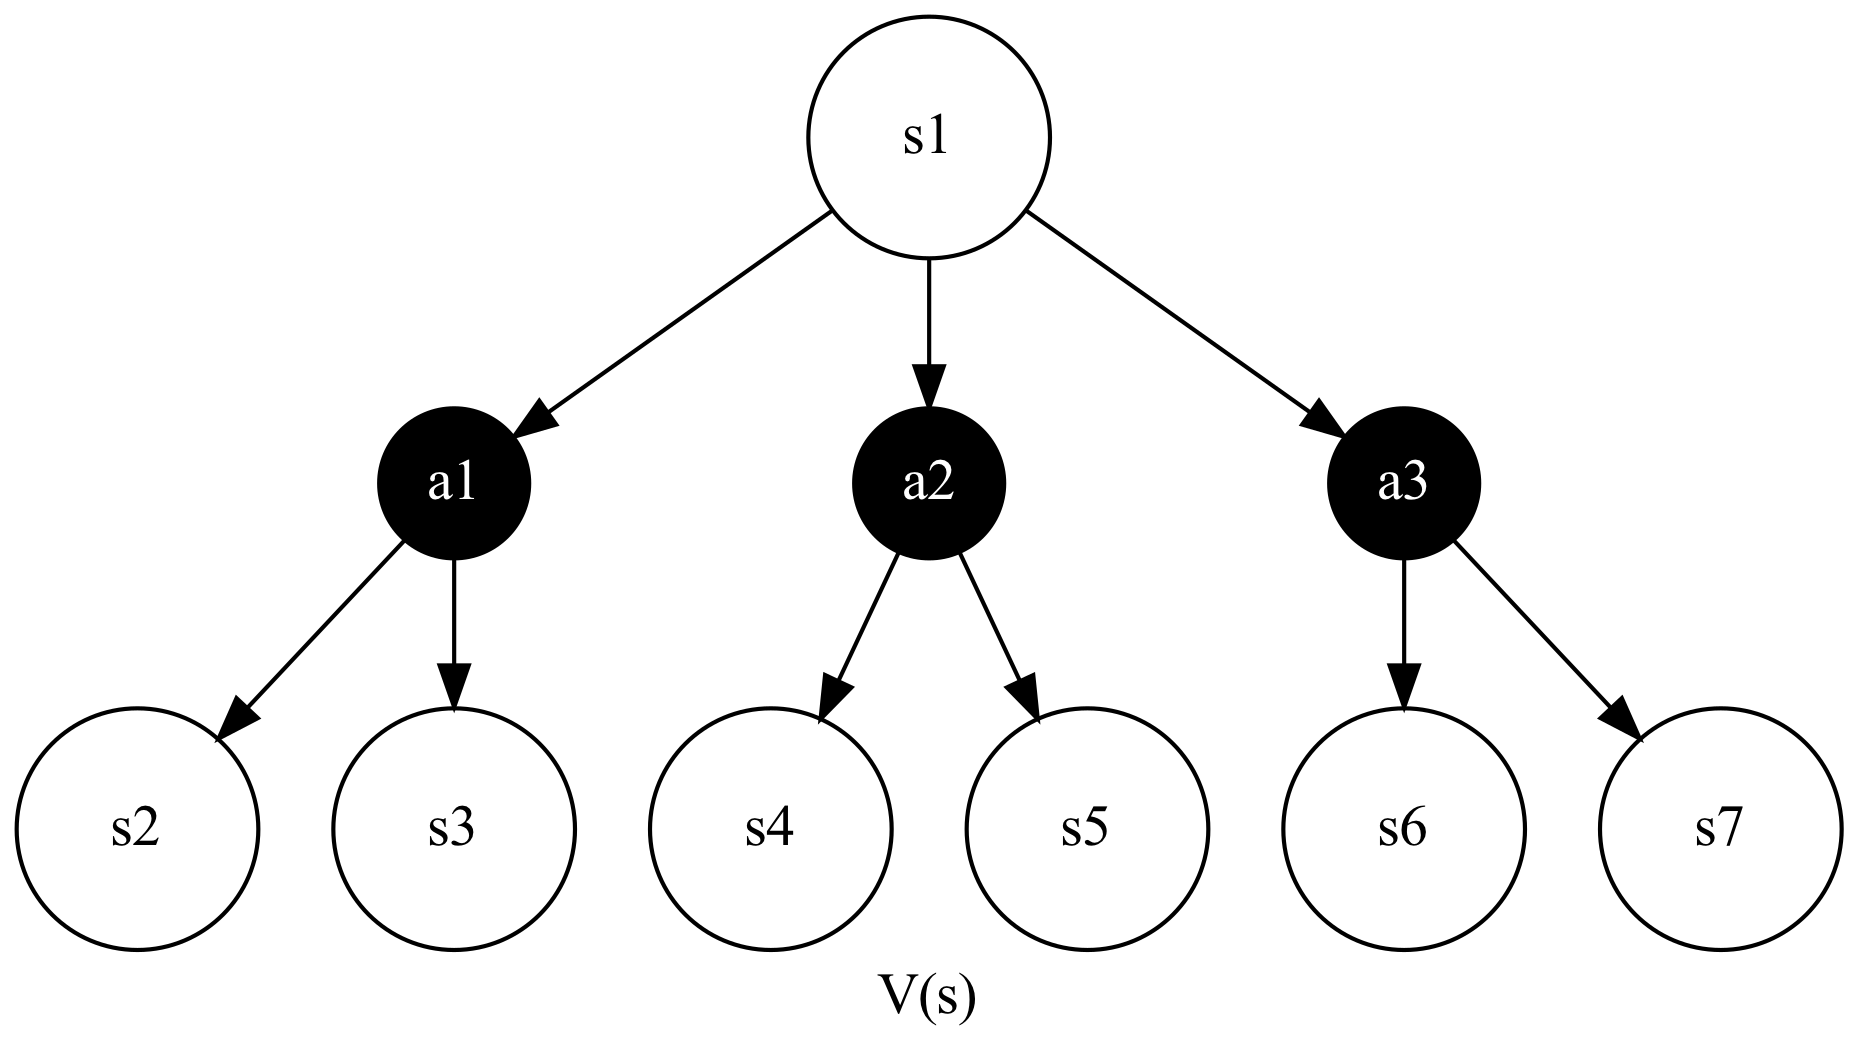
\includegraphics[width=7cm, height=4cm, keepaspectratio]{graphs/mc_td_6.png}
\end{center}
\end{column}
\begin{column}{.5\textwidth}
\begin{center}
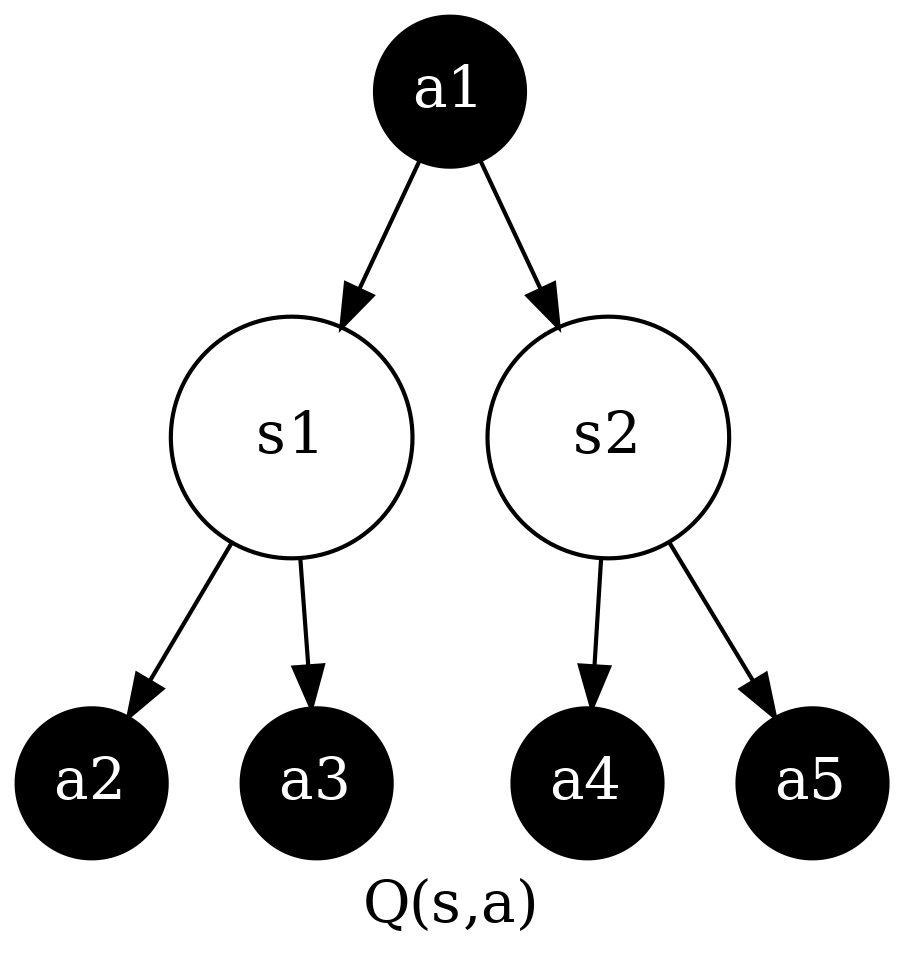
\includegraphics[width=7cm, height=4cm, keepaspectratio]{graphs/mc_td_7.png}
\end{center}
\end{column}
\end{columns}}
\only<2>{
\begin{center}
{\large Monte Carlo}
\end{center}
\begin{columns}
\begin{column}{.5\textwidth}
\begin{center}
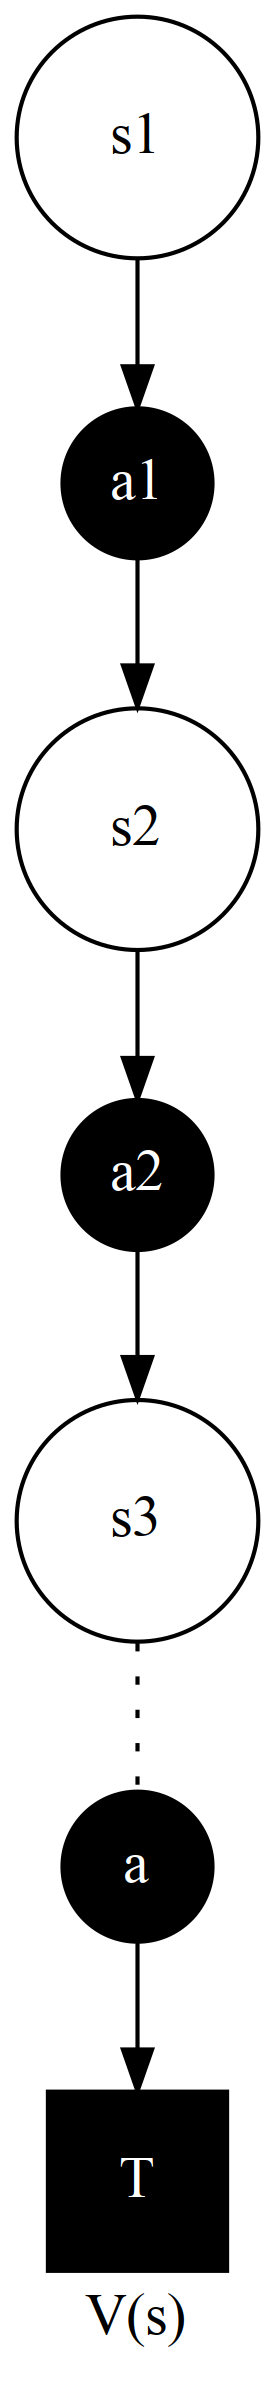
\includegraphics[width=7cm, height=6cm, keepaspectratio]{graphs/mc_td_2.png}
\end{center}
\end{column}
\begin{column}{.5\textwidth}
\begin{center}
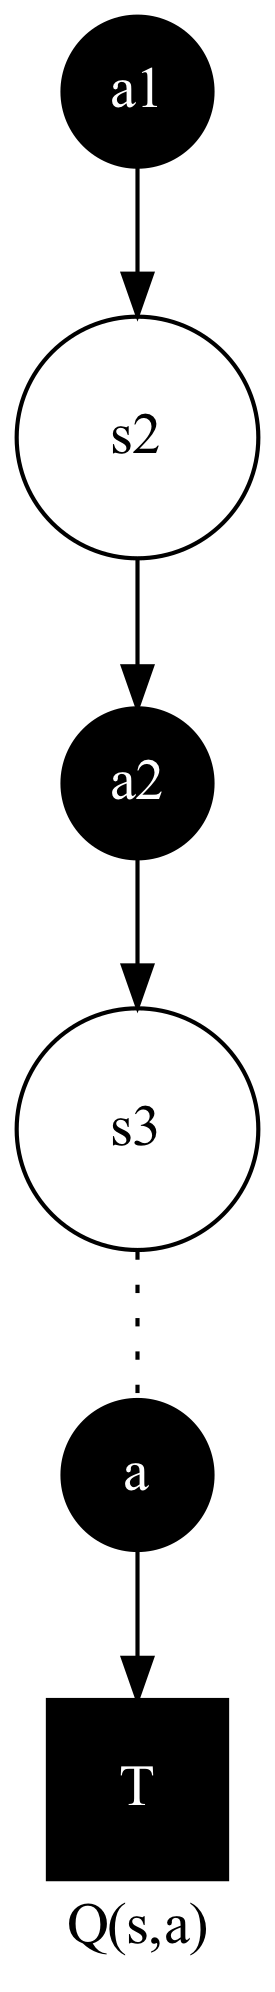
\includegraphics[width=7cm, height=6cm, keepaspectratio]{graphs/mc_td_3.png}
\end{center}
\end{column}
\end{columns}}
\only<3>{
\begin{center}
{\large Időbeli különbségek}
\end{center}
\begin{columns}
\begin{column}{.5\textwidth}
\begin{center}
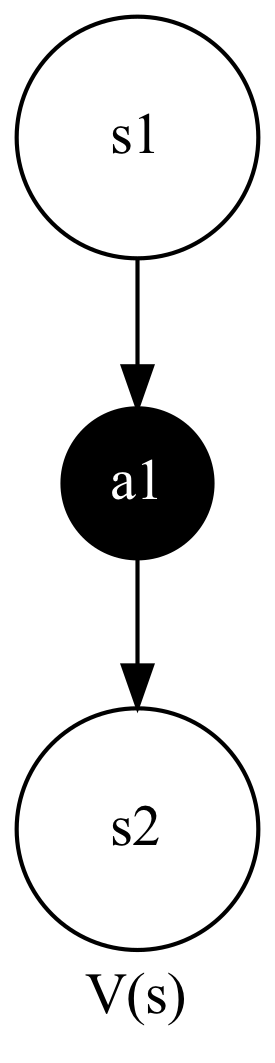
\includegraphics[width=7cm, height=5cm, keepaspectratio]{graphs/mc_td_4.png}
\end{center}
\end{column}
\begin{column}{.5\textwidth}
\begin{center}
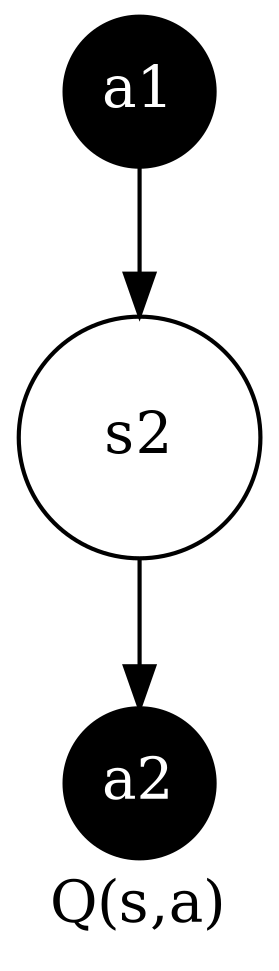
\includegraphics[width=7cm, height=5cm, keepaspectratio]{graphs/mc_td_5.png}
\end{center}
\end{column}
\end{columns}}
\only<4>{
\begin{center}
{\large $n$ lépéses különbségek}
\end{center}
\begin{columns}
\begin{column}{.5\textwidth}
\begin{center}
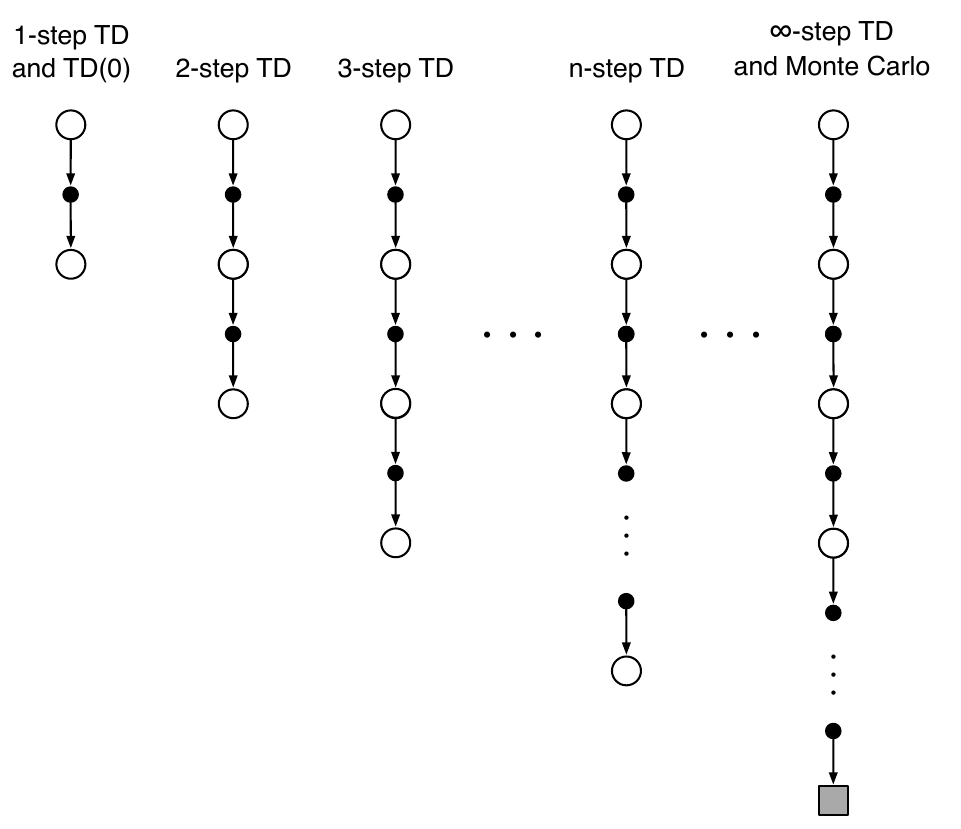
\includegraphics[width=7cm, height=5cm, keepaspectratio]{images/mc_td_14.png}
\end{center}
\end{column}
\begin{column}{.5\textwidth}
\begin{center}
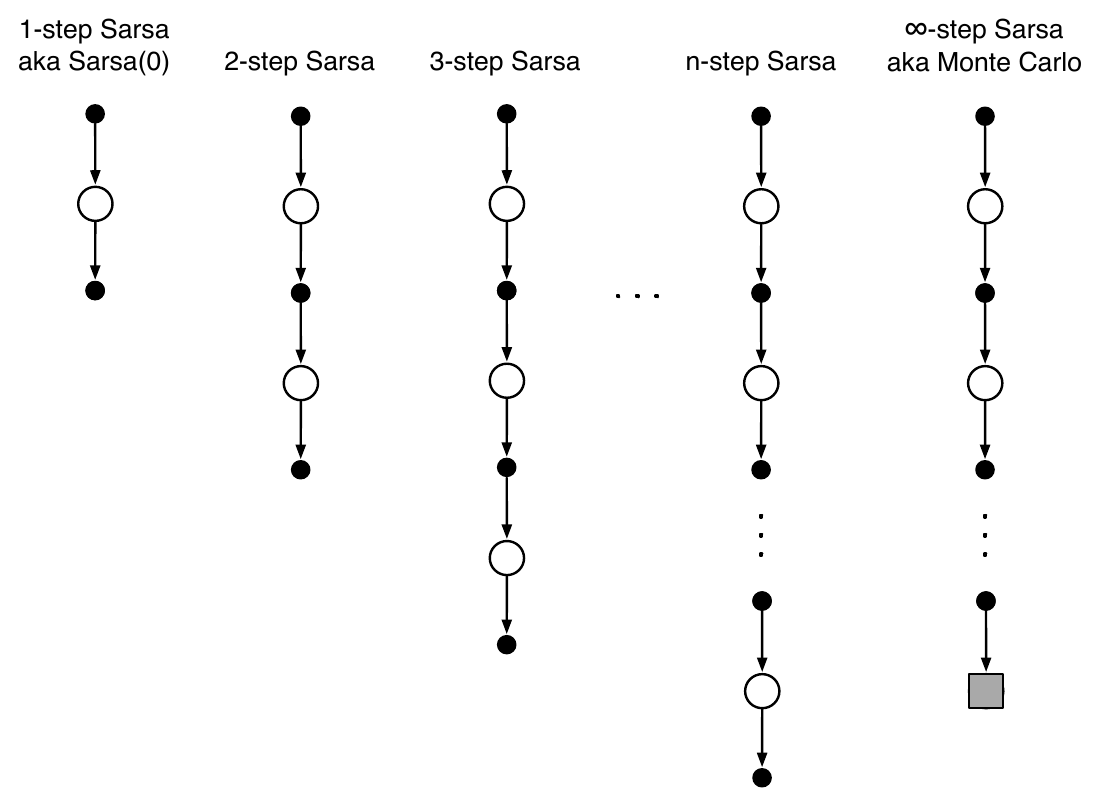
\includegraphics[width=7cm, height=5cm, keepaspectratio]{images/mc_td_16.png}
\end{center}
\end{column}
\end{columns}}
\end{frame}

\end{document}





















